\chapter{IDP-bestand resulterend uit de procedure beschreven in hoofdstuk \ref{sec:consistentie}}\label{app:consistentie}

\lstinputlisting[title=Theorie voor het diagram in figuur \ref{fig:diagram-voorbeeld}]{chap-rol-idp/generatedtheory.idp}\label{code:consistentie}

\chapter{IDP-bestand resulterend uit de procedure beschreven in hoofdstuk \ref{sec:kwaliteitsgebrek}}\label{app:kwaliteitsgebrek}

\lstinputlisting[title=Theorie voor het opsporen van kwaliteitsgebreken]{chap-rol-idp/defs.idp}\label{code:kwaliteitsgebrek}

\chapter{IDP-bestand voor sequentiediagram van het spelvoorbeeld}\label{app:seq-diagram-game}

\lstinputlisting[title=Modellering van het gedrag van het sequentiediagram in figuur \ref{fig:seq-diagram-game}]{idp-sources/seq-diagram-game.idp}\label{code:seq-diagram-game}

\chapter{IDP-bestand voor sequentiediagram voor het voorbeeld over recursie}\label{app:seq-recursion}

\lstinputlisting[title=Modellering van het gedrag van de sequentiediagrammen in figuren \ref{fig:methodOne} en \ref{fig:methodtwo}]{idp-sources/recursion.idp}\label{code:seq-recursion}

\chapter{IDP-bestand voor sequentiediagram voor het voorbeeld over extra instructies}\label{app:new-nim}

\lstinputlisting[title=Modellering van Nim gebruikmakend van nieuwe soorten instructies]{idp-sources/new-lang.idp}\label{code:new-nim}

\chapter{IDP-bestand voor het ontwerp van Nim}

\lstinputlisting[title=Modellering van Nim voor hoofdstuk \ref{sec:evaluatie}]{chap-evaluatie/nimmodel.idp}\label{code:nim-eval}

\chapter{Wetenschappelijk artikel}

\includepdf[pages=-]{IEEEtran/article.pdf}
%
%% bare_conf.tex
%% V1.4b
%% 2015/08/26
%% by Michael Shell
%% See:
%% http://www.michaelshell.org/
%% for current contact information.
%%
%% This is a skeleton file demonstrating the use of IEEEtran.cls
%% (requires IEEEtran.cls version 1.8b or later) with an IEEE
%% conference paper.
%%
%% Support sites:
%% http://www.michaelshell.org/tex/ieeetran/
%% http://www.ctan.org/pkg/ieeetran
%% and
%% http://www.ieee.org/

%%*************************************************************************
%% Legal Notice:
%% This code is offered as-is without any warranty either expressed or
%% implied; without even the implied warranty of MERCHANTABILITY or
%% FITNESS FOR A PARTICULAR PURPOSE! 
%% User assumes all risk.
%% In no event shall the IEEE or any contributor to this code be liable for
%% any damages or losses, including, but not limited to, incidental,
%% consequential, or any other damages, resulting from the use or misuse
%% of any information contained here.
%%
%% All comments are the opinions of their respective authors and are not
%% necessarily endorsed by the IEEE.
%%
%% This work is distributed under the LaTeX Project Public License (LPPL)
%% ( http://www.latex-project.org/ ) version 1.3, and may be freely used,
%% distributed and modified. A copy of the LPPL, version 1.3, is included
%% in the base LaTeX documentation of all distributions of LaTeX released
%% 2003/12/01 or later.
%% Retain all contribution notices and credits.
%% ** Modified files should be clearly indicated as such, including  **
%% ** renaming them and changing author support contact information. **
%%*************************************************************************


% *** Authors should verify (and, if needed, correct) their LaTeX system  ***
% *** with the testflow diagnostic prior to trusting their LaTeX platform ***
% *** with production work. The IEEE's font choices and paper sizes can   ***
% *** trigger bugs that do not appear when using other class files.       ***                          ***
% The testflow support page is at:
% http://www.michaelshell.org/tex/testflow/



\documentclass[conference]{IEEEtran}
% Some Computer Society conferences also require the compsoc mode option,
% but others use the standard conference format.
%
% If IEEEtran.cls has not been installed into the LaTeX system files,
% manually specify the path to it like:
% \documentclass[conference]{../sty/IEEEtran}





% Some very useful LaTeX packages include:
% (uncomment the ones you want to load)


% *** MISC UTILITY PACKAGES ***
%
%\usepackage{ifpdf}
% Heiko Oberdiek's ifpdf.sty is very useful if you need conditional
% compilation based on whether the output is pdf or dvi.
% usage:
% \ifpdf
%   % pdf code
% \else
%   % dvi code
% \fi
% The latest version of ifpdf.sty can be obtained from:
% http://www.ctan.org/pkg/ifpdf
% Also, note that IEEEtran.cls V1.7 and later provides a builtin
% \ifCLASSINFOpdf conditional that works the same way.
% When switching from latex to pdflatex and vice-versa, the compiler may
% have to be run twice to clear warning/error messages.






% *** CITATION PACKAGES ***
%
\usepackage{cite}
% cite.sty was written by Donald Arseneau
% V1.6 and later of IEEEtran pre-defines the format of the cite.sty package
% \cite{} output to follow that of the IEEE. Loading the cite package will
% result in citation numbers being automatically sorted and properly
% "compressed/ranged". e.g., [1], [9], [2], [7], [5], [6] without using
% cite.sty will become [1], [2], [5]--[7], [9] using cite.sty. cite.sty's
% \cite will automatically add leading space, if needed. Use cite.sty's
% noadjust option (cite.sty V3.8 and later) if you want to turn this off
% such as if a citation ever needs to be enclosed in parenthesis.
% cite.sty is already installed on most LaTeX systems. Be sure and use
% version 5.0 (2009-03-20) and later if using hyperref.sty.
% The latest version can be obtained at:
% http://www.ctan.org/pkg/cite
% The documentation is contained in the cite.sty file itself.






% *** GRAPHICS RELATED PACKAGES ***
%
\ifCLASSINFOpdf
  \usepackage[pdftex]{graphicx}
  % declare the path(s) where your graphic files are
  % \graphicspath{{../pdf/}{../jpeg/}}
  % and their extensions so you won't have to specify these with
  % every instance of \includegraphics
  \DeclareGraphicsExtensions{.pdf,.jpeg,.png}
\else
  % or other class option (dvipsone, dvipdf, if not using dvips). graphicx
  % will default to the driver specified in the system graphics.cfg if no
  % driver is specified.
  % \usepackage[dvips]{graphicx}
  % declare the path(s) where your graphic files are
  % \graphicspath{{../eps/}}
  % and their extensions so you won't have to specify these with
  % every instance of \includegraphics
  % \DeclareGraphicsExtensions{.eps}
\fi
% graphicx was written by David Carlisle and Sebastian Rahtz. It is
% required if you want graphics, photos, etc. graphicx.sty is already
% installed on most LaTeX systems. The latest version and documentation
% can be obtained at: 
% http://www.ctan.org/pkg/graphicx
% Another good source of documentation is "Using Imported Graphics in
% LaTeX2e" by Keith Reckdahl which can be found at:
% http://www.ctan.org/pkg/epslatex
%
% latex, and pdflatex in dvi mode, support graphics in encapsulated
% postscript (.eps) format. pdflatex in pdf mode supports graphics
% in .pdf, .jpeg, .png and .mps (metapost) formats. Users should ensure
% that all non-photo figures use a vector format (.eps, .pdf, .mps) and
% not a bitmapped formats (.jpeg, .png). The IEEE frowns on bitmapped formats
% which can result in "jaggedy"/blurry rendering of lines and letters as
% well as large increases in file sizes.
%
% You can find documentation about the pdfTeX application at:
% http://www.tug.org/applications/pdftex





% *** MATH PACKAGES ***
%
\usepackage{amsmath}
% A popular package from the American Mathematical Society that provides
% many useful and powerful commands for dealing with mathematics.
%
% Note that the amsmath package sets \interdisplaylinepenalty to 10000
% thus preventing page breaks from occurring within multiline equations. Use:
\interdisplaylinepenalty=2500
% after loading amsmath to restore such page breaks as IEEEtran.cls normally
% does. amsmath.sty is already installed on most LaTeX systems. The latest
% version and documentation can be obtained at:
% http://www.ctan.org/pkg/amsmath





% *** SPECIALIZED LIST PACKAGES ***
%
%\usepackage{algorithmic}
% algorithmic.sty was written by Peter Williams and Rogerio Brito.
% This package provides an algorithmic environment fo describing algorithms.
% You can use the algorithmic environment in-text or within a figure
% environment to provide for a floating algorithm. Do NOT use the algorithm
% floating environment provided by algorithm.sty (by the same authors) or
% algorithm2e.sty (by Christophe Fiorio) as the IEEE does not use dedicated
% algorithm float types and packages that provide these will not provide
% correct IEEE style captions. The latest version and documentation of
% algorithmic.sty can be obtained at:
% http://www.ctan.org/pkg/algorithms
% Also of interest may be the (relatively newer and more customizable)
% algorithmicx.sty package by Szasz Janos:
% http://www.ctan.org/pkg/algorithmicx




% *** ALIGNMENT PACKAGES ***
%
%\usepackage{array}
% Frank Mittelbach's and David Carlisle's array.sty patches and improves
% the standard LaTeX2e array and tabular environments to provide better
% appearance and additional user controls. As the default LaTeX2e table
% generation code is lacking to the point of almost being broken with
% respect to the quality of the end results, all users are strongly
% advised to use an enhanced (at the very least that provided by array.sty)
% set of table tools. array.sty is already installed on most systems. The
% latest version and documentation can be obtained at:
% http://www.ctan.org/pkg/array


% IEEEtran contains the IEEEeqnarray family of commands that can be used to
% generate multiline equations as well as matrices, tables, etc., of high
% quality.




% *** SUBFIGURE PACKAGES ***
%\ifCLASSOPTIONcompsoc
%  \usepackage[caption=false,font=normalsize,labelfont=sf,textfont=sf]{subfig}
%\else
\usepackage[caption=false,font=footnotesize]{subfig}
%\fi
% subfig.sty, written by Steven Douglas Cochran, is the modern replacement
% for subfigure.sty, the latter of which is no longer maintained and is
% incompatible with some LaTeX packages including fixltx2e. However,
% subfig.sty requires and automatically loads Axel Sommerfeldt's caption.sty
% which will override IEEEtran.cls' handling of captions and this will result
% in non-IEEE style figure/table captions. To prevent this problem, be sure
% and invoke subfig.sty's "caption=false" package option (available since
% subfig.sty version 1.3, 2005/06/28) as this is will preserve IEEEtran.cls
% handling of captions.
% Note that the Computer Society format requires a larger sans serif font
% than the serif footnote size font used in traditional IEEE formatting
% and thus the need to invoke different subfig.sty package options depending
% on whether compsoc mode has been enabled.
%
% The latest version and documentation of subfig.sty can be obtained at:
% http://www.ctan.org/pkg/subfig




% *** FLOAT PACKAGES ***
%
%\usepackage{fixltx2e}
% fixltx2e, the successor to the earlier fix2col.sty, was written by
% Frank Mittelbach and David Carlisle. This package corrects a few problems
% in the LaTeX2e kernel, the most notable of which is that in current
% LaTeX2e releases, the ordering of single and  column floats is not
% guaranteed to be preserved. Thus, an unpatched LaTeX2e can allow a
% single column figure to be placed prior to an earlier double column
% figure.
% Be aware that LaTeX2e kernels dated 2015 and later have fixltx2e.sty's
% corrections already built into the system in which case a warning will
% be issued if an attempt is made to load fixltx2e.sty as it is no longer
% needed.
% The latest version and documentation can be found at:
% http://www.ctan.org/pkg/fixltx2e


%\usepackage{stfloats}
% stfloats.sty was written by Sigitas Tolusis. This package gives LaTeX2e
% the ability to do double column floats at the bottom of the page as well
% as the top. (e.g., "\begin{figure*}[!b]" is not normally possible in
% LaTeX2e). It also provides a command:
%\fnbelowfloat
% to enable the placement of footnotes below bottom floats (the standard
% LaTeX2e kernel puts them above bottom floats). This is an invasive package
% which rewrites many portions of the LaTeX2e float routines. It may not work
% with other packages that modify the LaTeX2e float routines. The latest
% version and documentation can be obtained at:
% http://www.ctan.org/pkg/stfloats
% Do not use the stfloats baselinefloat ability as the IEEE does not allow
% \baselineskip to stretch. Authors submitting work to the IEEE should note
% that the IEEE rarely uses double column equations and that authors should try
% to avoid such use. Do not be tempted to use the cuted.sty or midfloat.sty
% packages (also by Sigitas Tolusis) as the IEEE does not format its papers in
% such ways.
% Do not attempt to use stfloats with fixltx2e as they are incompatible.
% Instead, use Morten Hogholm'a dblfloatfix which combines the features
% of both fixltx2e and stfloats:
%
% \usepackage{dblfloatfix}
% The latest version can be found at:
% http://www.ctan.org/pkg/dblfloatfix




% *** PDF, URL AND HYPERLINK PACKAGES ***
%
%\usepackage{url}
% url.sty was written by Donald Arseneau. It provides better support for
% handling and breaking URLs. url.sty is already installed on most LaTeX
% systems. The latest version and documentation can be obtained at:
% http://www.ctan.org/pkg/url
% Basically, \url{my_url_here}.




% *** Do not adjust lengths that control margins, column widths, etc. ***
% *** Do not use packages that alter fonts (such as pslatex).         ***
% There should be no need to do such things with IEEEtran.cls V1.6 and later.
% (Unless specifically asked to do so by the journal or conference you plan
% to submit to, of course. )


% correct bad hyphenation here

\usepackage{todo}

\hyphenation{op-tical net-works semi-conduc-tor}


\begin{document}
%
% paper title
% Titles are generally capitalized except for words such as a, an, and, as,
% at, but, by, for, in, nor, of, on, or, the, to and up, which are usually
% not capitalized unless they are the first or last word of the title.
% Linebreaks \\ can be used within to get better formatting as desired.
% Do not put math or special symbols in the title.
\title{Translating UML Class Diagrams and Sequence Diagrams to FO($\cdot$) to Facilitate Simulation and Verification}


% author names and affiliations
% use a multiple column layout for up to three different
% affiliations
\author{\IEEEauthorblockN{Thomas Vochten}
\IEEEauthorblockA{Department of Computer Science\\
Katholieke Universiteit Leuven}}
% conference papers do not typically use \thanks and this command
% is locked out in conference mode. If really needed, such as for
% the acknowledgment of grants, issue a \IEEEoverridecommandlockouts
% after \documentclass

% for over three affiliations, or if they all won't fit within the width
% of the page, use this alternative format:
% 
%\author{\IEEEauthorblockN{Michael Shell\IEEEauthorrefmark{1},
%Homer Simpson\IEEEauthorrefmark{2},
%James Kirk\IEEEauthorrefmark{3}, 
%Montgomery Scott\IEEEauthorrefmark{3} and
%Eldon Tyrell\IEEEauthorrefmark{4}}
%\IEEEauthorblockA{\IEEEauthorrefmark{1}School of Electrical and Computer Engineering\\
%Georgia Institute of Technology,
%Atlanta, Georgia 30332--0250\\ Email: see http://www.michaelshell.org/contact.html}
%\IEEEauthorblockA{\IEEEauthorrefmark{2}Twentieth Century Fox, Springfield, USA\\
%Email: homer@thesimpsons.com}
%\IEEEauthorblockA{\IEEEauthorrefmark{3}Starfleet Academy, San Francisco, California 96678-2391\\
%Telephone: (800) 555--1212, Fax: (888) 555--1212}
%\IEEEauthorblockA{\IEEEauthorrefmark{4}Tyrell Inc., 123 Replicant Street, Los Angeles, California 90210--4321}}




% use for special paper notices
%\IEEEspecialpapernotice{(Invited Paper)}




% make the title area
\maketitle

% As a general rule, do not put math, special symbols or citations
% in the abstract
\begin{abstract}
Representing UML diagrams in logic can benefit a designer since the designer can easily miss errors or inefficiencies in the design if the diagrams grow sufficiently elaborate or numerous. In this article, we show a method to translate class diagrams and a corresponding set of sequence diagrams that model the behavior of a desired software system to FO($\cdot$), an extension of first-order predicate logic with inductive definitions, partial functions, aggregates and types. We show how the output theory may be used to verify consistency of a class diagram and detect the presence of certain design flaws in the class diagram. In addition, we show that the theory may be used to simulate system behavior as modelled in the sequence diagrams and how to verify that requirements regarding the output of a diagram are satisfied. We also evaluate performance in terms of execution time and the size of the grounding for each of these tasks.
\end{abstract}

% no keywords




% For peer review papers, you can put extra information on the cover
% page as needed:
% \ifCLASSOPTIONpeerreview
% \begin{center} \bfseries EDICS Category: 3-BBND \end{center}
% \fi
%
% For peerreview papers, this IEEEtran command inserts a page break and
% creates the second title. It will be ignored for other modes.
\IEEEpeerreviewmaketitle



\section{Introduction}
% no \IEEEPARstart
UML\cite{RumbaughJames2005Tuml} is a modelling language used in software engineering to graphically model a design for a software system. Popular types of diagrams are the class diagram and the sequence diagram. However, when a class diagram grows too elaborate or the sequence diagrams too numerous, the designer can easily miss any design errors or flaws or unintended behavior. Since errors made in the design phase can be costly to correct if found late in the software production process, automated verification of consistency and detection of the presence of design flaws might help the designer spot issues they might otherwise miss.

In this article we show a method to translate class diagrams and sequence diagrams that specify the behavior of methods defined in the corresponding class diagram to FO($\cdot$)\cite{DeCatBroes2014PLaa}, an extension of first-order logic with inductive definitions, aggregates, partial functions and types.

We will use a translation of a class diagram to verify whether the diagram is consistent, i.e. whether the FO($\cdot$) theory corresponding to the diagram has a model. We will also use an alternative translation to detect certain types of design flaws which make it more difficult to gain a clear understanding of a class diagram.

We will use a translation of a set of sequence diagrams to simulate the behavior modelled therein. We will then use that translation to verify whether the diagrams fulfill certain requirements.

The software we use to verify consistency, detect design flaws, simulate sequence diagrams and verify requirements for sequence diagrams is IDP\cite{DeCatBroes2014PLaa}, a knowledge base system for FO($\cdot$). IDP can perform model expansion, progression inference and other forms of inference given one or more input vocabularies, theories and structures. 

The rest of this article is structured as follows. Section \ref{sec:related-work} gives an overview of related work with regard to translating UML diagrams to logic. Section \ref{sec:class-diagram} introduces a method to translate class diagrams to FO($\cdot$) and verifies consistency of and detects design flaws in an example diagram. Section \ref{sec:seq} describes our method to translate a set of sequence diagrams to FO($\cdot$). Section \ref{sec:evaluation} evaluates the use of our method to design a set of diagrams that models the game Nim, whether the translation can be used to simulate the game and to verify whether certain requirements hold, and performance in terms of execution time and grounding size. Finally, section \ref{sec:conclusion} concludes the article.
% You must have at least 2 lines in the paragraph with the drop letter
% (should never be an issue)

\section{Related work}\label{sec:related-work}

This section provides an overview of previous work on translating UML diagrams to several kinds of logic.

In \cite{BerardiDaniela2005RoUc}, the authors first provide a method to translate class diagrams to FO-theories. The vocabulary first defines: Predicates that express membership of a class; predicates that relate instances of a class to their respective values for class attributes; predicates that model operations on a class by relating the callee object, values for parameters and the result value corresponding to that callee object and those parameters values; and predicates that relate objects of a class to objects of another class according to associations defined in the class diagram. The rules contained in the output theory make use of the membership predicates to enforce correct typing for the other kinds of predicates and ensure that the predicates for attributes, operations and associations obey the multiplicites imposed on them by the diagrams. Finally, the theory models inheritance by introducing rules that state that all members of a subclass must also be members of the superclass. Note that these inheritance rules do not prevent members of one class being members of another class even if the diagram defines no inheritance relationship between those two classes, regardless of whether the developer wants to allow for that possibility. The rest of the paper describes a method to translate class diagrams to several kinds of description logics and how to use those translations to verify consistency of the diagram and to detect implicit properties which unintentionally hold in the diagram. In this article, we adapt the method for translating class diagrams to FO introduced by the authors to make use of logical types, thereby removing the need to introduce rules in the output theory that enforce the correct typing and rules that model inheritance.

In \cite{KuhlmannMirco2012FUaO}, the authors briefly introduce relational logic and outline how to translate class diagrams to relational logic by defining constants that represent instances of a class and binary relations that relate constants according to attribute and association relationships. The translation imposes conditions on membership of the relations in order to enforce correct typing and multiplicites defined in the diagram. They also show how to translate constraints expressed in OCL\cite{WarmerJosB1999Ocl:}. The authors describe how they use Kodkod\cite{10.1007/978-3-540-71209-1_49} to calculate instances of an output relational model. Kodkod translates relational models to SAT-formulas and translates solutions in SAT format back to solutions for the relational model.

In \cite{LIMA2009143}, the authors describe how to represent sequence diagrams in PROMELA\cite{neumann2014using}, a modelling language that models processes. PROMELA is used by the SPIN\cite{holzmann2004spin} model checker to verify whether properties expressed in linear temporal logic (LTL) hold in the modelled processes. It is possible to simulate sequence diagrams with the proposed representation. The paper also describes how to represent state transitions during the execution of a sequence diagram by listing the performed action, the lifeline that performed the action, the message and the lifeline that sent/received the message for each time step. The authors present a sequence diagram that models the behavior of an ATM in order to prove they can verify certain properties for a sequence diagram. They express four properties in LTL. SPIN determines that only one property holds. For the other three properties, SPIN generates a counterexample of an execution of the sequence diagram that violates the property. However, the authors consider sequence diagrams independently from any class diagram. Therefore, their method cannot truly represent a system of which the state may change over time. They also do not consider sequence diagrams that call other sequence diagrams. Full understanding of a system may only be gained by considering that type of sequence diagram.

Every work discussed in this section uses a subset of FO to perform verification and certain forms of inference on UML class diagrams. Sequence diagrams are considered separately. Our contribution is to instead use FO($\cdot$) to both model class and sequence diagrams and to perform verification on those diagrams.

One cannot express transitive closure in FO in a general manner and hence also not in these subsets of FO. However, transitive closures are easily expressible in FO($\cdot$), and hence it can also correctly specify inheritance relationships. 

We prefer sequence diagrams to activity diagrams since the former allow the use of variables internal to a specific diagram.


\section{Translating class diagrams to FO($\cdot$)}\label{sec:class-diagram}

In this section, we adapt the method to translate class diagrams to FO introduced in \cite{BerardiDaniela2005RoUc} to make use of logical types. We will use the diagram in figure \ref{fig:game-class} to illustrate how we translate class diagrams to FO($\cdot$).

\subsection{Building a theory for checking consistency}\label{sec:consistency}

\begin{figure*}[!t]
\centering
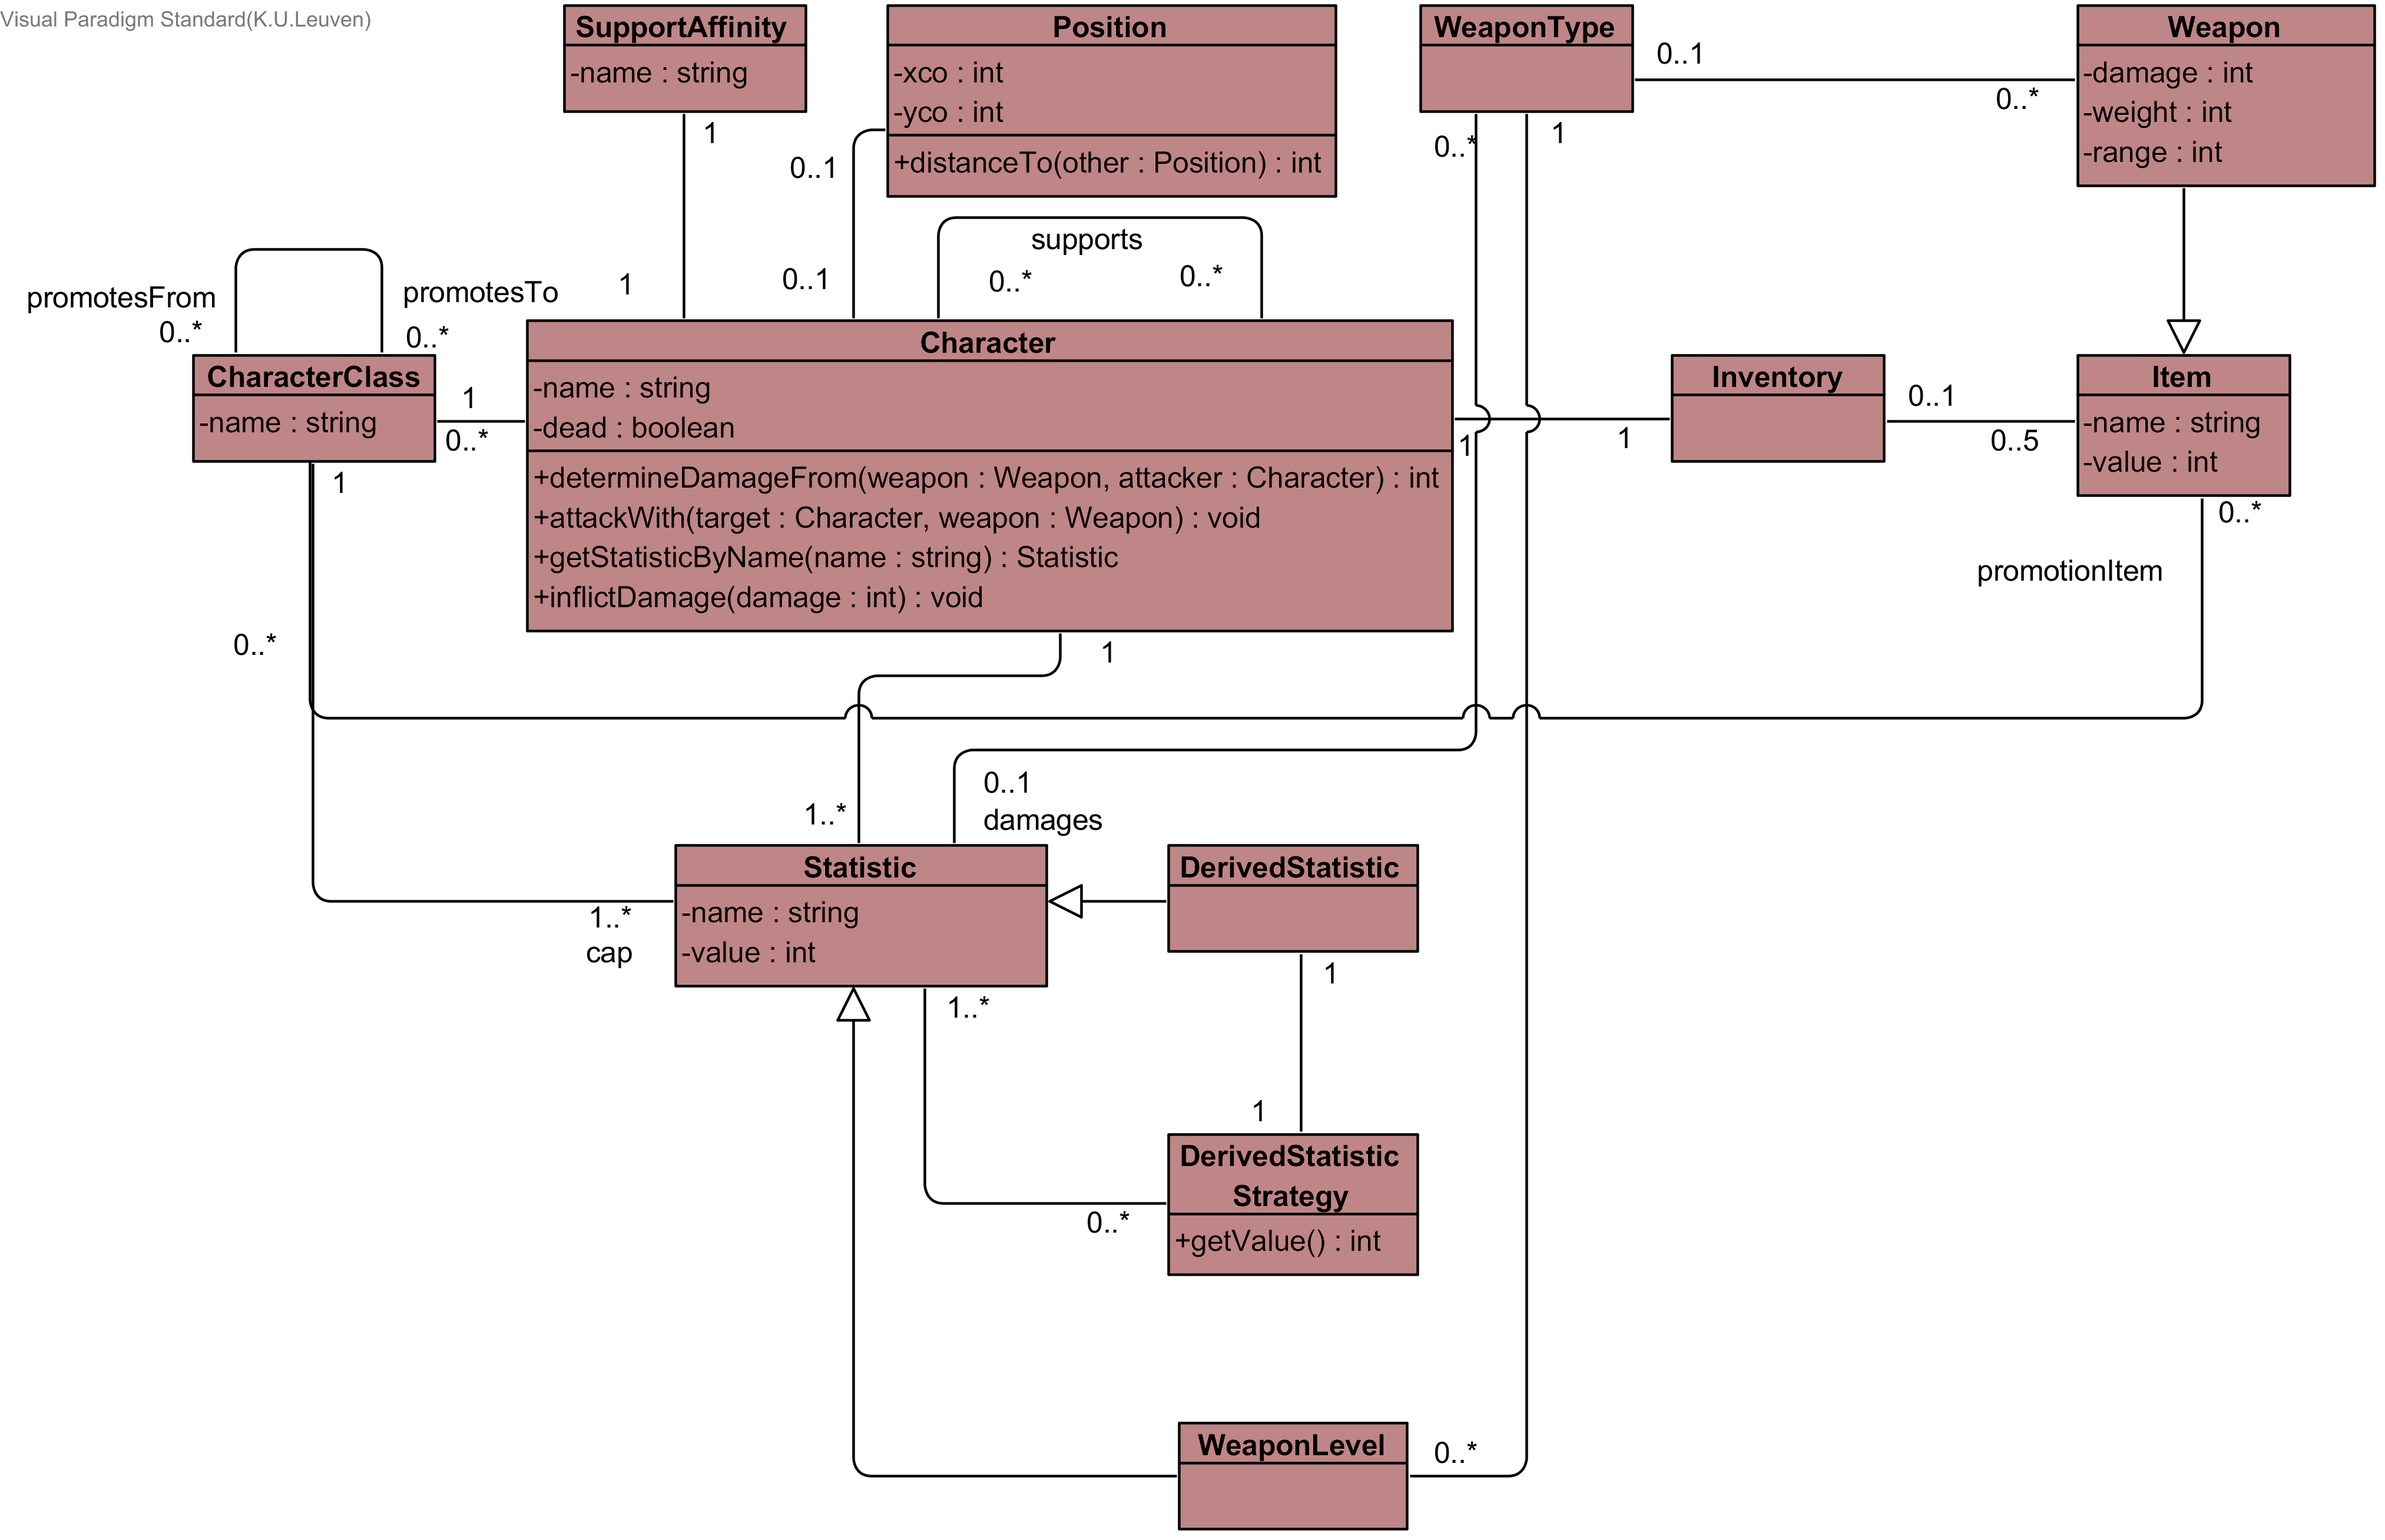
\includegraphics[width=0.75\textwidth]{diagram-voorbeeld}
\caption{Example class diagram}
\label{fig:game-class}
\end{figure*}

Every class is represented by a logical type. In order to enforce correct typing for every predicate we introduce, we need merely specify the correct logical type corresponding to the class expected for each predicate argument.

We introduce a binary predicate for every class attribute and we name it according to the pattern \textit{Classnameattributename}. For example, the predicate corresponding to \textit{name} in \textit{Character} is \textit{Charactername(Character, string)}. In addition, we introduce rules which enforce the multiplicity imposed on the pattern according to the following general pattern:

\begin{align*}
	&\forall{o1}[ClassType](lowerBound \leq \#\{o2[attributeType] : \\ &Classnameattributename(o1, o2)\} \leq upperBound).
\end{align*}

For \textit{name} in \textit{Character}, we get:

\begin{align*}
	\forall{o1}[Character]\exists!{o2}[string](Charactername(o1, o2)).
\end{align*}

We deviate from \cite{BerardiDaniela2005RoUc} by not introducing predicates corresponding to class operations, since sequence diagrams should model the behavior of operations.

For each association, we introduce an $m$-ary predicate where $m$ equals the amount of classes involved in the association. We name them according to the pattern \textit{ClassOneand$\cdots$andClassM(ClassOne, $\cdots$, ClassM)}. The association between \textit{Inventory} and \textit{Item} thus yields \textit{InventoryandItem(Inventory, Item)}. Again, we enforce multiplicity by introducing rules for each role of each association according to the following general pattern:

\begin{align*}
	&\forall{c_1}[Class_1]\cdots{}\forall{c_m}[Class_m](lowerBound_l \leq \\ &\#\{o_l[Class_l] : ClassOneand\cdots{}andClassM\\&(c_1, \cdots, o_l, \cdots, c_m)\} \leq upperBound_l).
\end{align*}

where $l$ indicates the role for which the multiplicity is being enforced. This yields the following two rules for the \textit{Inventory}---\textit{Item} association:

\begin{align*}
	&\forall{o2}[Item](\#\{o1[Inventory] : \\ &InventoryandItem(o1, o2)\} \leq 1). \\
	&\forall{o1}[Inventory](\#\{o2[Item] : \\ &InventoryandItem(o1, o2)\} \leq 5).
\end{align*}

To model inheritance, the vocabulary must simply declare that logical types corresponding to a subclass are subtypes of the logical type corresponding to the superclass. This means that every input structure for the output theory must include all members of the interpretation of a subtype in the interpretation of all the corresponding supertypes in order to be valid input for model expansion. It is possible to spare the user this inconvenience by abandoning the principle of one logical type per class and instead introducing a general logical type \textit{Object} and introducing another logical type \textit{ClassObject} which has one object for every class. We would then add a binary predicate \textit{StaticClass(ClassObject, Object)} in order to express membership of a class. Inductive definitions would then use the inheritance relationships contained in the diagram to calculate the correct class memberships for every object. However, this approach would require rewriting every rule introduced earlier in this section to be longer by enforcing correct typing, which would make the output theory more difficult to understand. There would also have to be additional rules to enforce the correct type for every argument of every attribute and association predicate. For these reasons, we chose not to implement this approach.

We have used these rules to automatically generate an FO($\cdot$) theory based on the diagram in figure \ref{fig:game-class}. Given a valid input structure, IDP found a model. The conclusion is therefore that the diagram is consistent.

\subsection{Building a theory for detecting design flaws}\label{sec:design-flaw}

In order to detect design flaws, we need a separate theory where the classes themselves take center stage instead of specific instances of those classes. Therefore, we remove the logical types for each class and use the \textit{ClassObject} logical type we rejected in the previous subsection. We also introduce the predicates \textit{IsDirectSupertypeOf(ClassObject, ClassObject)} and \textit{IsSupertypeOf(ClassObject, ClassObject)} predicates. The former expresses a direct inheritance relationship while the latter is the transitive closure over \textit{IsDirectSupertypeOf/2}. We model that transitive closure in the following inductive definition:

\begin{align*}
	\{ &\forall{x}[ClassObject]\forall{y}[ClassObject](IsSupertypeOf(x, y) \\ &\leftarrow IsDirectSupertypeOf(x, y)). \\
	&\forall{x}[ClassObject]\forall{y}[ClassObject](IsSupertypeOf(y, x) \\ &\leftarrow \exists{z}[ClassObject](IsSupertypeOf(y, z)  \\ &\land IsSupertypeOf(z, x))).\}
\end{align*}

A separate inductive definition then fills in \textit{IsDirectSupertypeOf/2} with direct inheritance relationships read from the diagram.

In this article, we consider three different kinds of design flaws related to associations:

\begin{itemize}
	\item \textbf{Many-to-many associations}: The presence of a many-to-many association is generally an indication that there is a class missing from the design.
	\item \textbf{Loose class}: If a class cannot be reached by navigating associations, that class is essentially useless and should be eliminated.
	\item \textbf{Insufficiently precise upper bound in a multiplicity}\cite{Balaban2015}: Consider figure \ref{fig:design-flaw}. The multiplicities imply that classes \textit{Alice}, \textit{Bob} and \textit{Charlie} contain an equal number of instances. This renders the upper bound of 2 on \textit{Alice} in \textit{Charlie}---\textit{Alice} insufficiently precise since the other bounds imply that every instance of \textit{Charlie} is associated with exactly one instance of \textit{Alice}. Since this fact is not immediately apparent, such a bound should be corrected to improve the understandability of the diagram. Either set the upper bound on \textit{Alice} to 1, set the lower bound on \textit{Alice} to 0 or increase the upper bound on \textit{Charlie}.
\end{itemize}

\begin{figure}[!t]
	\centering
	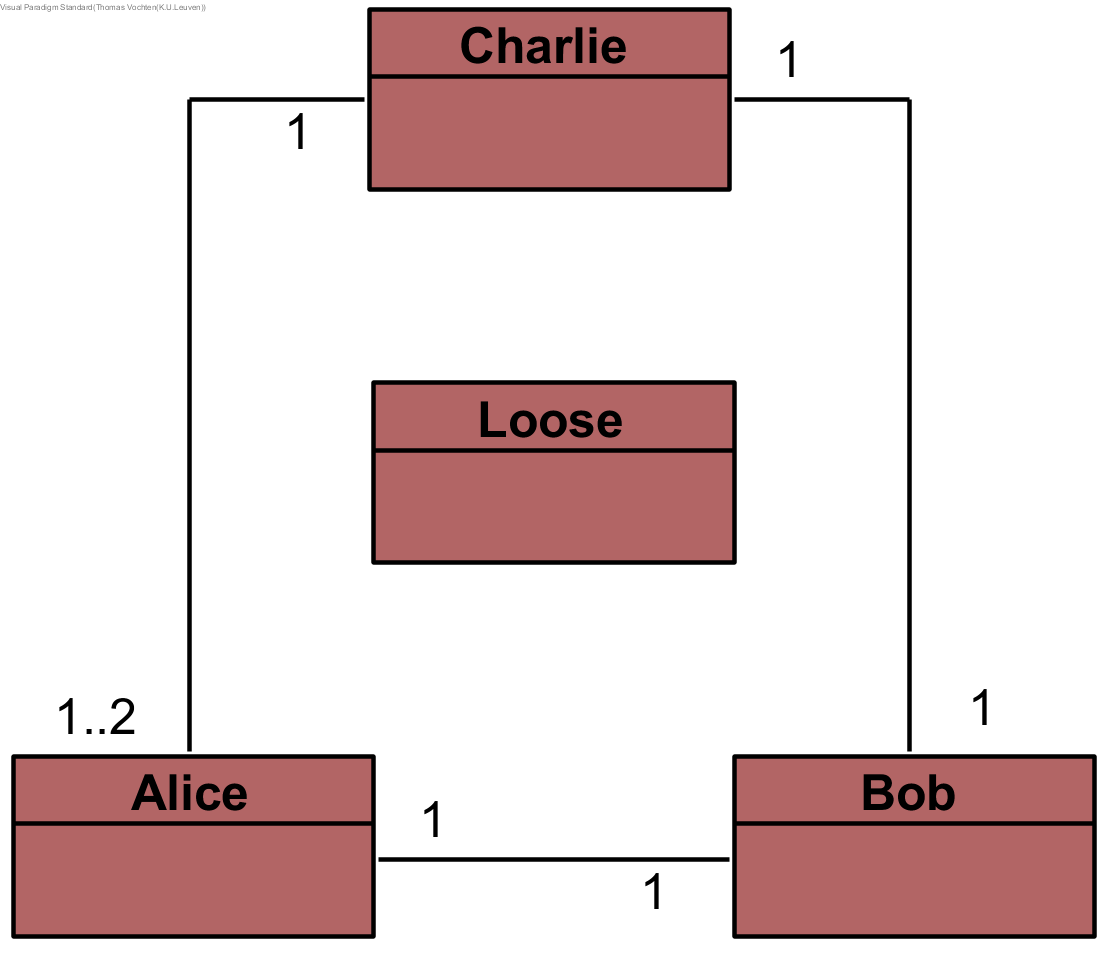
\includegraphics[width=2in]{cycle}
	\caption{Example of loose class and insufficiently precise multiplicity upper bound}
	\label{fig:design-flaw}
\end{figure}

We introduce three other predicates in order to encode information about binary associations.

\textit{BiAssoc(ClassObject, ClassObject)} expresses that a binary association exists between two classes.

\textit{BiAssocLow(ClassObject, ClassObject, ClassObject, nat)} indicates that the role corresponding to the class named in the third argument has the lower bound specified in the fourth argument.

Similarly, \textit{BiAssocHigh(ClassObject, ClassObject, ClassObject, nat)} specifies the upper bound for the role corresponding to the argument parameter.

For the first two named design flaws, we introduce the following two rules:

\begin{align}
	\nonumber &\forall{x}[ClassObject]\forall{y}[ClassObject](ManyToMany(x, y) \\ \nonumber &\Leftrightarrow BiAssoc(x, y) \land \lnot \exists{z}[nat](BiAssocHigh(x, y, x, z)) \\ &\land \lnot \exists{z}[nat](BiAssocHigh(x, y, y, z))).\label{form:flaw1} \\
	\nonumber &\forall{x}[ClassObject](LooseClass(x) \Leftrightarrow \\ \nonumber &\lnot (\exists{y}[ClassObject](\lnot(x = y) \land (BiAssoc(x, y) \\ \nonumber  &\lor \exists{s}[ClassObject]\exists{y}[ClassObject]\\ &(IsSupertypeOf(s, x) \land BiAssoc(s, y)))))).\label{form:flaw2} \\
	&\nonumber\forall{x}[ClassObject]\forall{y}[ClassObject] \\
	&\nonumber(CycleImpreciseUpperBound(x, y, x) \\ &\nonumber\Leftrightarrow EqualNbInstances(x, y) \land BiAssocLow(x, y, x) \\ &\nonumber= BiAssocHigh(x, y, y) = BiAssocLow(x, y, y) \\ &\nonumber\land (BiAssocHigh(x, y, x) > BiAssocLow(x, y, x) \\ &\lor \lnot\exists{z}[nat](BiAssocHigh(x, y, x) = z))).\label{form:flaw3}
\end{align}

Rule \ref{form:flaw1} designates an association as many-to-many if neither role specifies an upper bound.

Rule \ref{form:flaw2} designates a class as loose if it is not directly associated with another class or if it does not have a superclass that is directly associated with another class.

Rule \ref{form:flaw3} designates an upper bound as insufficiently precise if the association is between two classes with an equal number of instances and if the other three bounds are both equal to each other and less than the considered upper bound. \textit{EqualNbInstances/2} is a helper predicate that expresses that two classes must have an equal number of instances. We construct the interpretation of this predicate by way of transitive closure over associations for which all bounds are equal.

We combine the information from the diagrams in figures \ref{fig:game-class} and \ref{fig:design-flaw} into one theory. IDP finds all many-to-many associations, concludes that \textit{Loose} is a loose class and the upper bound on \textit{Alice} in \textit{Charlie}---\textit{Alice} is insufficiently precise.

\section{Translating sequence diagrams to FO($\cdot$)}\label{sec:seq}
We will use the framework of linear time calculus\cite{BogaertsBart2014Sdsu} (LTC). LTC can model dynamic systems that change over time. Across each time step, only the inertial predicates that need be changed to the diagram do so, while all other inertial predicates remain the same. If we model diagram variables, an instruction pointer, a stack level counter and a return point stack as inertial predicates, we have exactly the elements we need to translate mutually recursive sequence diagrams to FO($\cdot$) theories.

In this section, we first describe how to expand the vocabulary and theory generated according to the rules described in section \ref{sec:consistency} in order to implement the elements summed up in the previous paragraph.

We introduce the following logical types and logical symbols to the vocabulary:

\begin{itemize}
	\item \textit{SDPoint}: This serves as an instruction pointer. It is a constructed type that consists of labels for all instructions across all given sequence diagrams, landing points after each call to a sequence diagram, and additional hidden last instructions we add for sequence diagrams that model methods that return \textit{void}. \textit{SDPoint}s are named according to the pattern \textit{$diagramname\_\langle{}sequencenumber\rangle$}, except landing points after diagram calls, which are named according to \textit{$diagramname\_\langle{}sequencenumber\rangle$post}
	\item \textit{NextSD(SDPoint) : SDPoint}: A partial function that specifies which \textit{SDPoint} follows the given \textit{SDPoint}. All \textit{SDPoint}s except the last instruction for each diagram are members of the domain.
	\item \textit{SDPointAt(Time, SDPoint)}: The \textit{SDPoint} at any given time step.
	\item \textit{StackLevel}: A non-zero natural number that indicates the stack depth.
	\item \textit{CurrentStackLevel(Time) : StackLevel}: A total function which specifies what the stack depth is at any given time step.
	\item \textit{ReturnPoint(Time, StackLevel, SDPoint)}: This predicate contains the return instruction at the specified stack depth. If the execution reaches the final instruction of a diagram, the instruction counter should be set to the corresponding \textit{SDPoint} at the following time step.
	\item Predicates for every diagram variable named according to the pattern \textit{VariableNameT(Time, StackLevel, VariableType)}. These diagram variables include variables defined in an instruction, lifeline objects and arguments of calls.
\end{itemize}

In addition, we modify the predicates corresponding to class variables to take logical type \textit{Time} as an additional argument. At this time, we do not allow the interpretation for association predicates to vary over time.

We follow the method outlined in \cite{BogaertsBart2014Sdsu} to make the logical symbols \textit{SDPointAt/2}, \textit{CurrentStackLevel/1} and \textit{ReturnPoint/3} inertial, as well as all diagram variable predicates and class variable predicates. Only class variable predicates have a corresponding \textit{uncause} predicate, since we allow only class variables to have more than one value at any given time step. If a diagram specifies an upper bound equal to one for the multiplicity of a class variable, that class variable may still have only one value at any given time step.

With these logical symbols, predicates and functions at our disposal, we are now equipped to translate sequence diagrams to FO($\cdot$) theories. Consider figure \ref{fig:recursion}. Diagram \ref{fig:methodOne} calls diagram \ref{fig:methodTwo}, whereupon diagram \ref{fig:methodTwo} calls itself two times and then returns. In this case, the members of \textit{SDPoint} are \textit{methodOne\_1}, \textit{methodOne\_2}, \textit{methodOne\_3}, \textit{methodOne\_3post}, \textit{methodOne\_4}, the hidden final instruction \textit{methodOne\_5}, \textit{methodTwo\_1}, \textit{methodTwo\_2}, \textit{methodTwo\_3}, \textit{methodTwo\_3post}, \textit{methodTwo\_4} and hidden final instruction \textit{methodTwo\_5}. We introduce the inertial predicates \textit{ObjT/3}, \textit{Obj2T/3}, \textit{FinishedT/3} and \textit{MTwoArgT/3}. We add causation rules corresponding to each instruction that contains an assignment to a variable or an object call. In the latter case, we add causation rules that set the correct callee object, call arguments, ensure that the value for \textit{SDPointAt/2} is the first instruction of the called diagram and set the return instruction for the next stack level to the hidden landing point after the call instruction. We also add causation rules corresponding to the final instruction of each diagram where the return instruction for the current stack depth is retrieved and set to be the value of \textit{SDPointAt/2} at the next time step. If any diagram modelled a non-void method, then we would add a causation rule corresponding to the landing point after a call of that diagram where the returned value is retrieved and is set to be the value of the assigned variable.

\begin{figure*}[!t]
\centering
\subfloat[Example of calling another diagram]{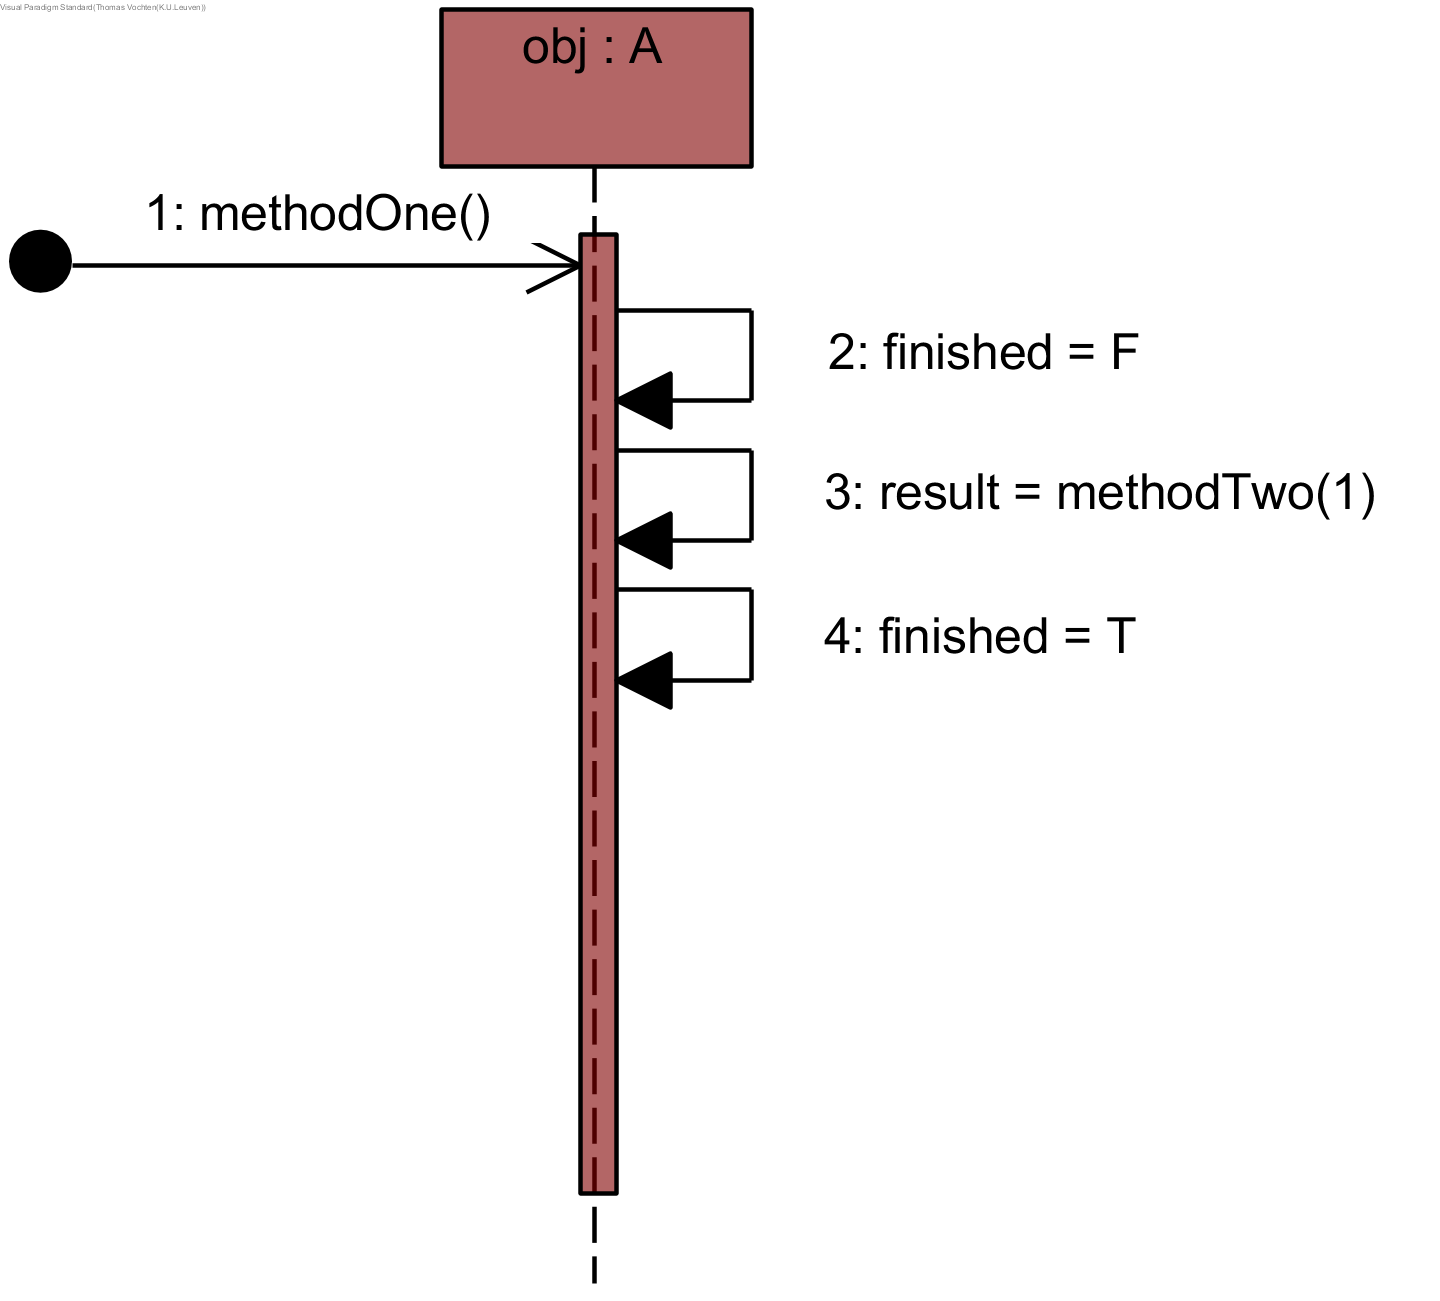
\includegraphics[width=0.325\textwidth]{methodOne}%
\label{fig:methodOne}}
\hfil
\subfloat[Example of recursion]{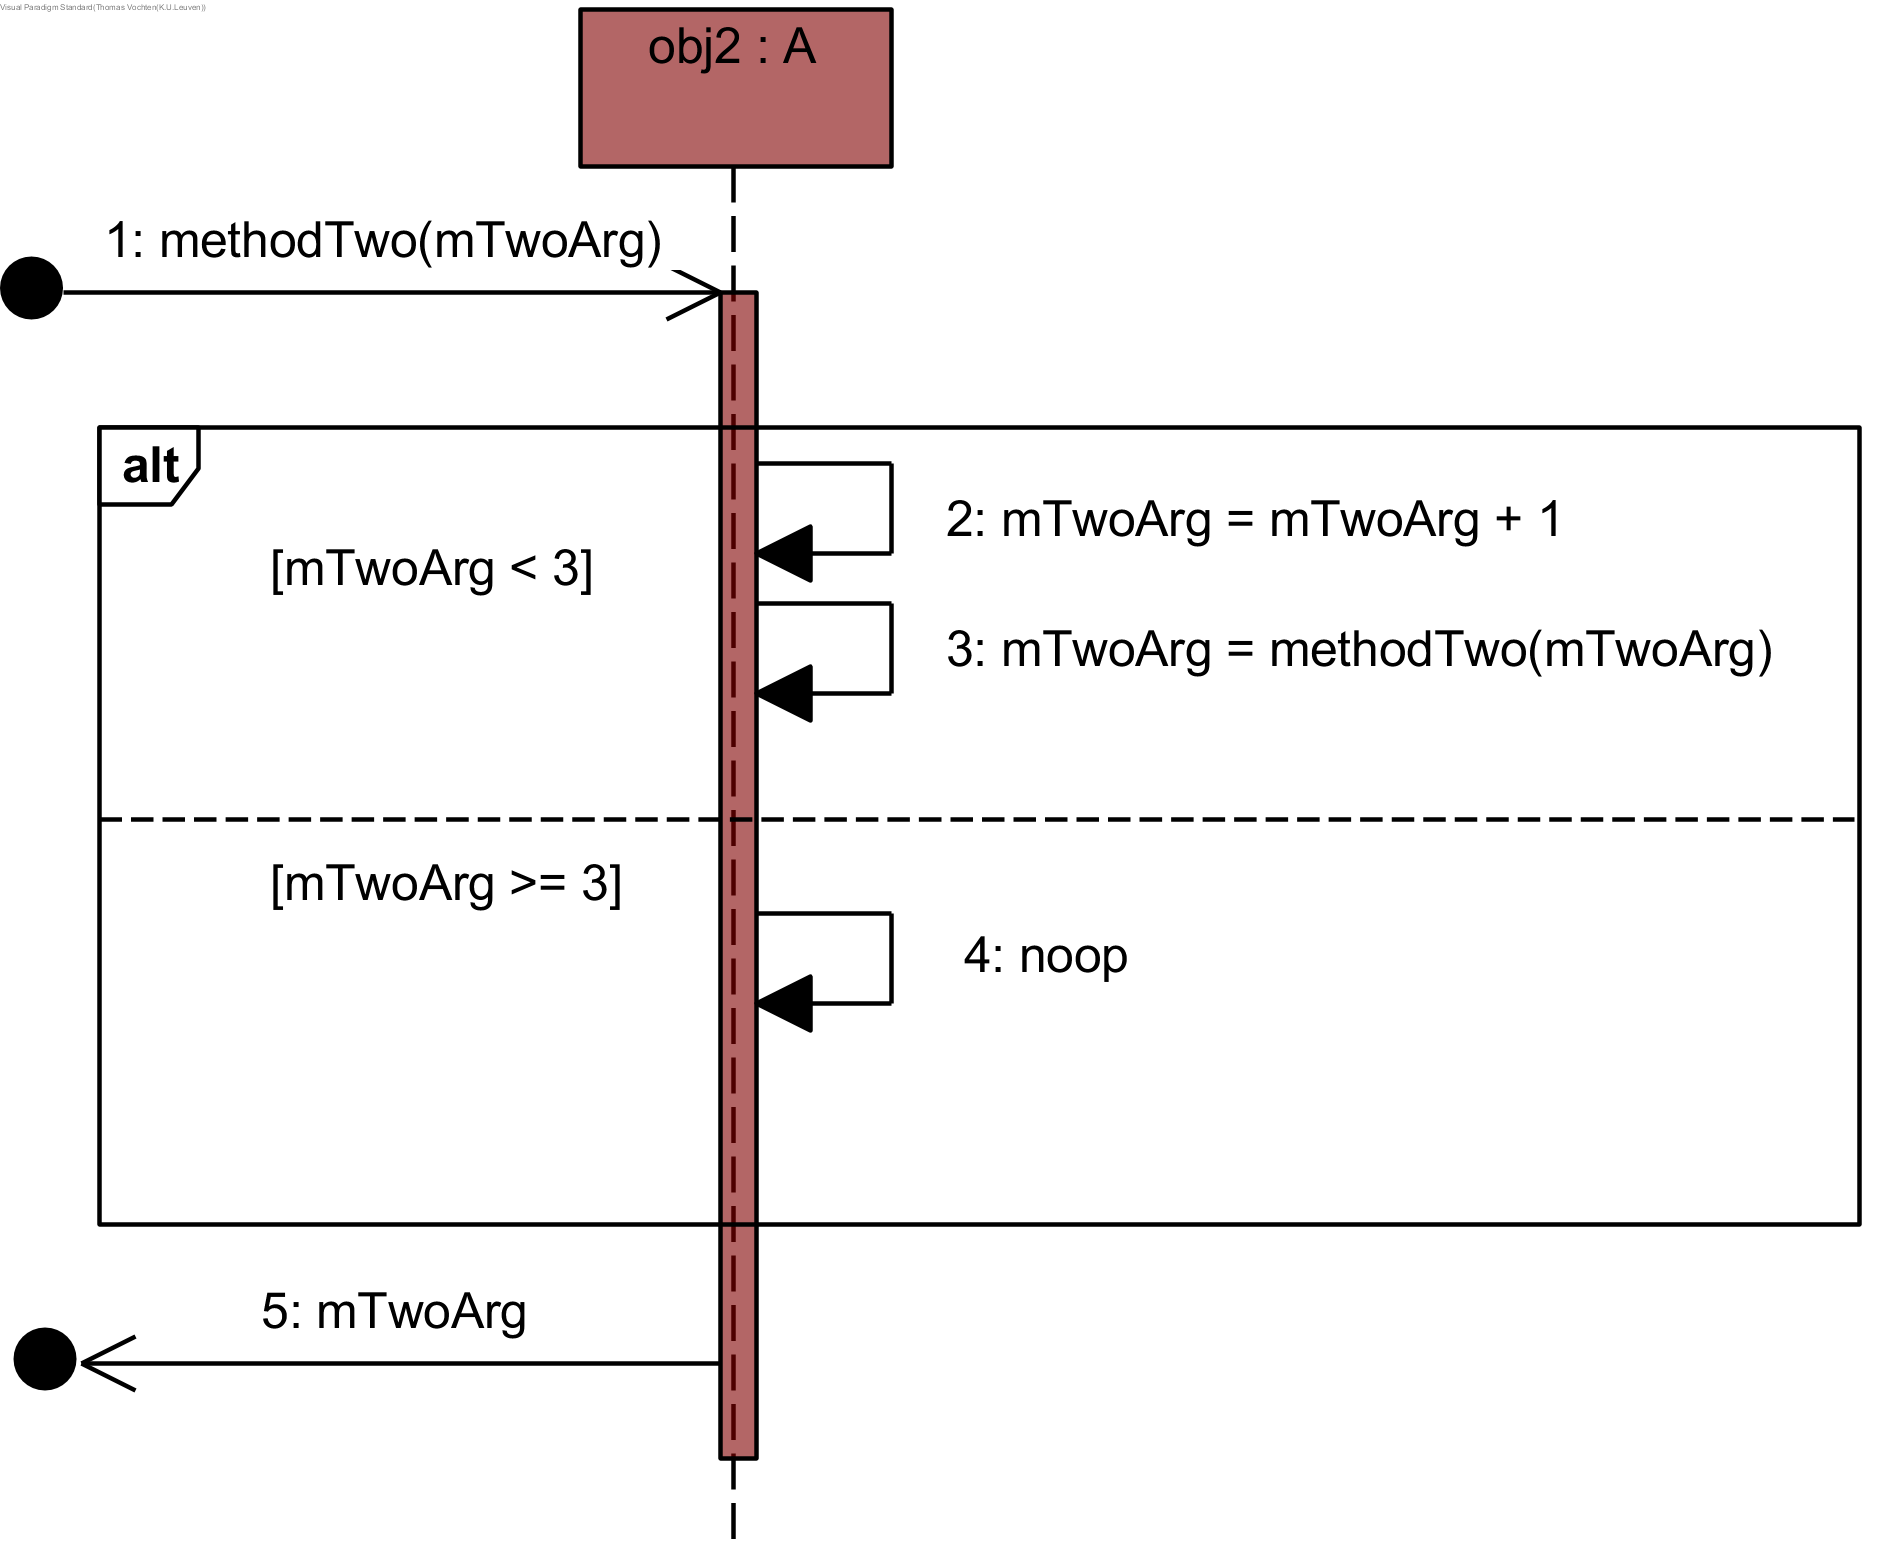
\includegraphics[width=0.4\textwidth]{methodTwo}%
\label{fig:methodTwo}}
\caption{Example of a set of sequence diagrams}
\label{fig:recursion}
\end{figure*}

With regard to \textit{SDPointAt/2}, we add a causation rule specifying that every \textit{SDPoint} is always followed by the \textit{SDPoint} named in \textit{NextSD/1} for that \textit{SDPoint}, except if that \textit{SDPoint} corresponds to a diagram call, the final instruction of a diagram or if it precedes a combined fragment. We have already discussed call instructions and final instructions of a diagram. We have designed elaborate algorithms that output the correct causation rules related to combined fragments, but we will only outline our general approach in this article.

We consider only alt combined fragments and loop combined fragments, which respectively correspond to an \textit{if}-\textit{else}-structure and a loop structure.

If the execution is about to enter a combined fragment, then we wish to determine in a single step which instruction the execution should jump to. In order to facilitate this, we have need of three algorithms:

\begin{itemize}
	\item Given a combined fragment, return the instructions the execution might jump to when entering the fragment and which conditions should hold for the jump to each instruction. Make the distinction between the \textit{if} and \textit{else} parts of an alt combined fragment.
	\item Given a combined fragment, determine all possible final instructions of the fragment and return all instructions the execution might jump to from each of those final instructions and which conditions, if any, should hold in order to make that jump.
	\item Given a combined fragment, determine all possible final instructions and check for loop combined fragments that the execution might re-enter. Return all instructions the execution might jump to and which conditions should hold in order to make that jump.
\end{itemize} 

Each of these algorithms should account for the fact that combined fragments might be nested and that the execution skips over loop combined fragments if their associated condition does not hold.

The general approach with regard to parsing combined fragment then goes as follows. If the message immediately preceding the combined fragment currently under consideration is not part of a combined fragment, then determine which are the first possible messages of this fragment and note that the execution jumps from that preceding message to those first messages if their corresponding conditions hold. If the immediately preceding message is part of a combined fragment, then determine the possible exit instructions for that combined fragment and use that information to determine which final messages for the preceding fragment jump to which possible first messages for the current fragment under which conditions. Finally, check if the current fragment is a loop combined fragment and/or is nested in one or more loop combined fragments and determine what instructions the execution might jump to when re-entering the loops. The output of this procedure is a set of causation rules for \textit{SDPointAt/3}.

We now have a set of rules that allows us to automatically generate a theory that accurately captures the behavior modelled in a set of mutually recursive sequence diagrams.

\section{Evaluation of translation from sequence diagrams to FO($\cdot$) theory}\label{sec:evaluation}

In this section, we will design a class diagram and a set of sequence diagrams that model the game of Nim. We will evaluate the difficulty of the design process. We will also evaluate the performance of simulation using the output theory and of verification of certain requirements using model expansion with respect to execution time and memory usage in terms of virtual memory usage for the simulation and grounding size for the verifications.

\subsection{Evaluation of the design}
Figures \ref{fig:nim-cd-play}, \ref{fig:ahe-ie} and \ref{fig:tt-take} contain the class diagram and sequence diagrams for our model of Nim. Nim is a fairly simple game, which means that the only real difficulty was designing a workaround for changing an object's association relations not being allowed during execution. This is why the class \textit{Game} has variables \textit{gameFinished} and \textit{p1Win}. These are a substitute for having a class \textit{Player} and an association \textit{Game}---\textit{Player} that designates a winner. Other limitations that contributed to making the diagrams longer than they otherwise could have been were that every alt combined fragment must have both an \textit{if} branch and an \textit{else} branch, and also that object call instructions must not contain expressions that require evaluation more complex than variable retrieval.

\subsection{Evaluation of simulation}

We simulated a game with two heaps. One of the heaps contains two objects and the other contains three objects. The first player removes all three objects from the second heap. The second player then removes one object from the first heap. Finally, the first player has no choice but to remove the last object and loses.
Table \ref{tab:sim-mem} contains the virtual memory usage at the start of each turn. It shows how simulating a game will require several gigabytes of memory.

Figure \ref{fig:boxplot} shows a boxplot of the execution time per time step, and figure \ref{fig:boxplot-nooutliers} shows a boxplot of the same data with the outliers removed. Half of the data lies between approximately 6.65 seconds and 6.9 seconds. Figure \ref{fig:boxplot-nooutliers} also shows the vast majority of the data is spread between approximately 6.5 seconds and 7.15 seconds. This distribution does lead to the total duration of the game being slightly less than 19 minutes, since the simulation was 116 steps long.

\subsection{Evaluation of verification for requirements}

The requirements we tested for are whether \textit{isEmpty()} returns true if and only if the heap the method is called on contains zero objects and whether \textit{allHeapsEmpty()} returns true if and only if all heaps are empty. To test this, we wrote four theories for each diagram which we each merge with the output theory one at a time for a total of four runs per diagram, one for each of these sentences:

\begin{itemize}
	\item The result is true while the heap is not empty/not all heaps are empty.
	\item The result is false while the heap is empty/all heaps are empty.
	\item The result is true while the heap is empty/all heaps are empty.
	\item The result is false while the heap is not empty/not all heaps are empty.
\end{itemize}

The expectation for both diagrams is that the first two sentences lead to an unsatisfiable theory, while the third and fourth sentences lead IDP to answer with the expected models. The third sentence for \textit{isEmpty()} should lead IDP to answer with the model corresponding to an empty heap while the fourth sentence should lead to an answer with all models corresponding to non-empty heaps. Similarly, the third sentence for \textit{allHeapsEmpty()} should lead to an answer with the model corresponding to all heaps being empty and the fourth sentence should lead to an answer with all models corresponding to at least one non-empty heap.

The input structure for \textit{isEmpty()} specifies that there are seven time steps in total, while for \textit{allHeapsEmpty()}, there are 25 time steps in total. Each run did indeed lead to the expected answer. For each diagram, the runs were similar in terms of execution time and grounding size. For \textit{isEmpty()}, the execution time is approximately 40 seconds, the size of the grounding is 578,306 and memory usage is 2.14 GB. For \textit{allHeapsEmpty()} given two heaps, the execution time is approximately 43.29 seconds, the grounding size is 366,643 and memory usage is 1.63 GB.

\begin{figure*}[!t]
	\centering
	\subfloat[Class diagram for Nim]{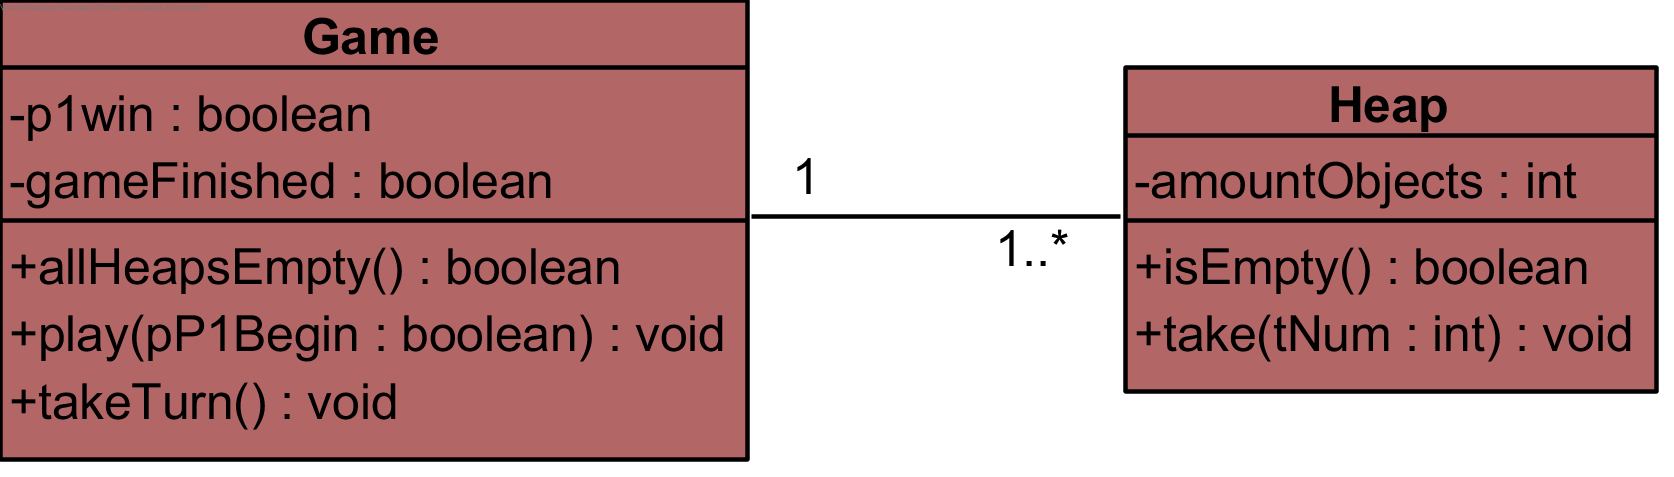
\includegraphics[width=0.5\textwidth]{ClassDiagram1}%
		\label{fig:nim-cd}}
	\hfil
	\subfloat[Sequence diagram for \textit{play()}]{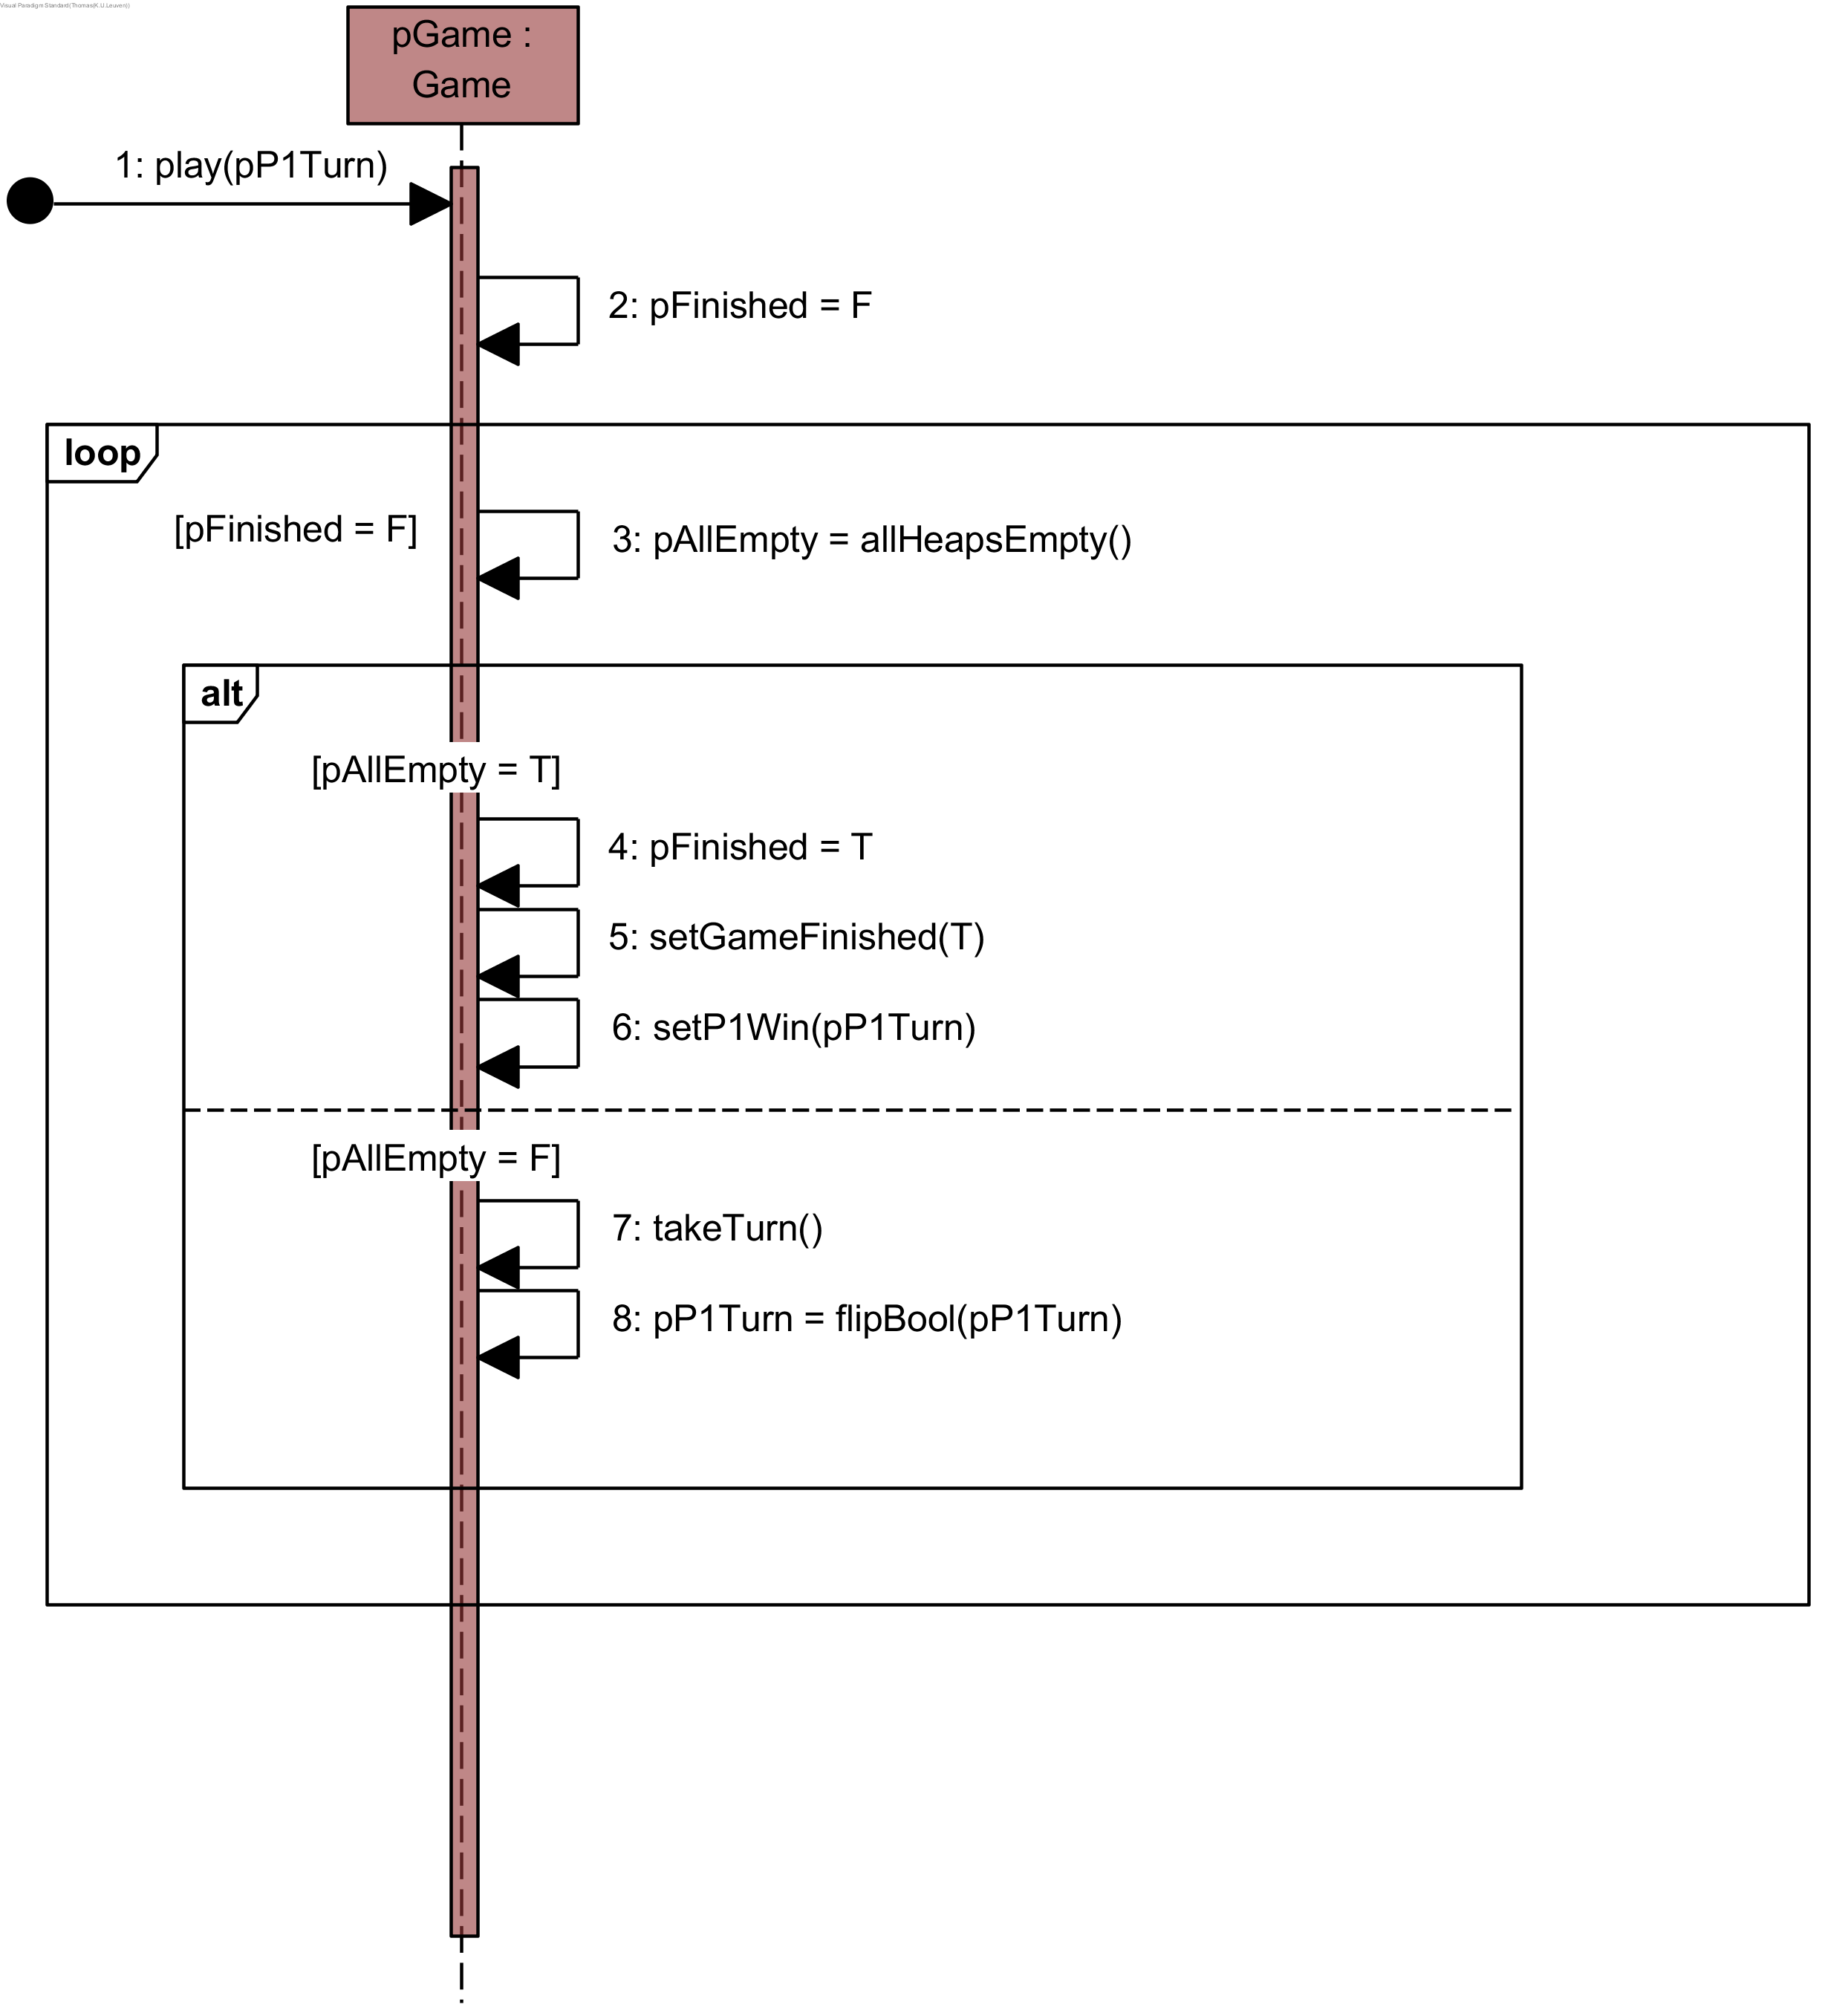
\includegraphics[width=0.5\textwidth]{play}}%
		\label{fig:play}
	\caption{Class diagram for Nim and sequence diagram for \textit{play()}}
	\label{fig:nim-cd-play}
\end{figure*}

\begin{figure*}[!t]
	\centering
	\subfloat[Sequence diagram from \textit{allHeapsEmpty()}]{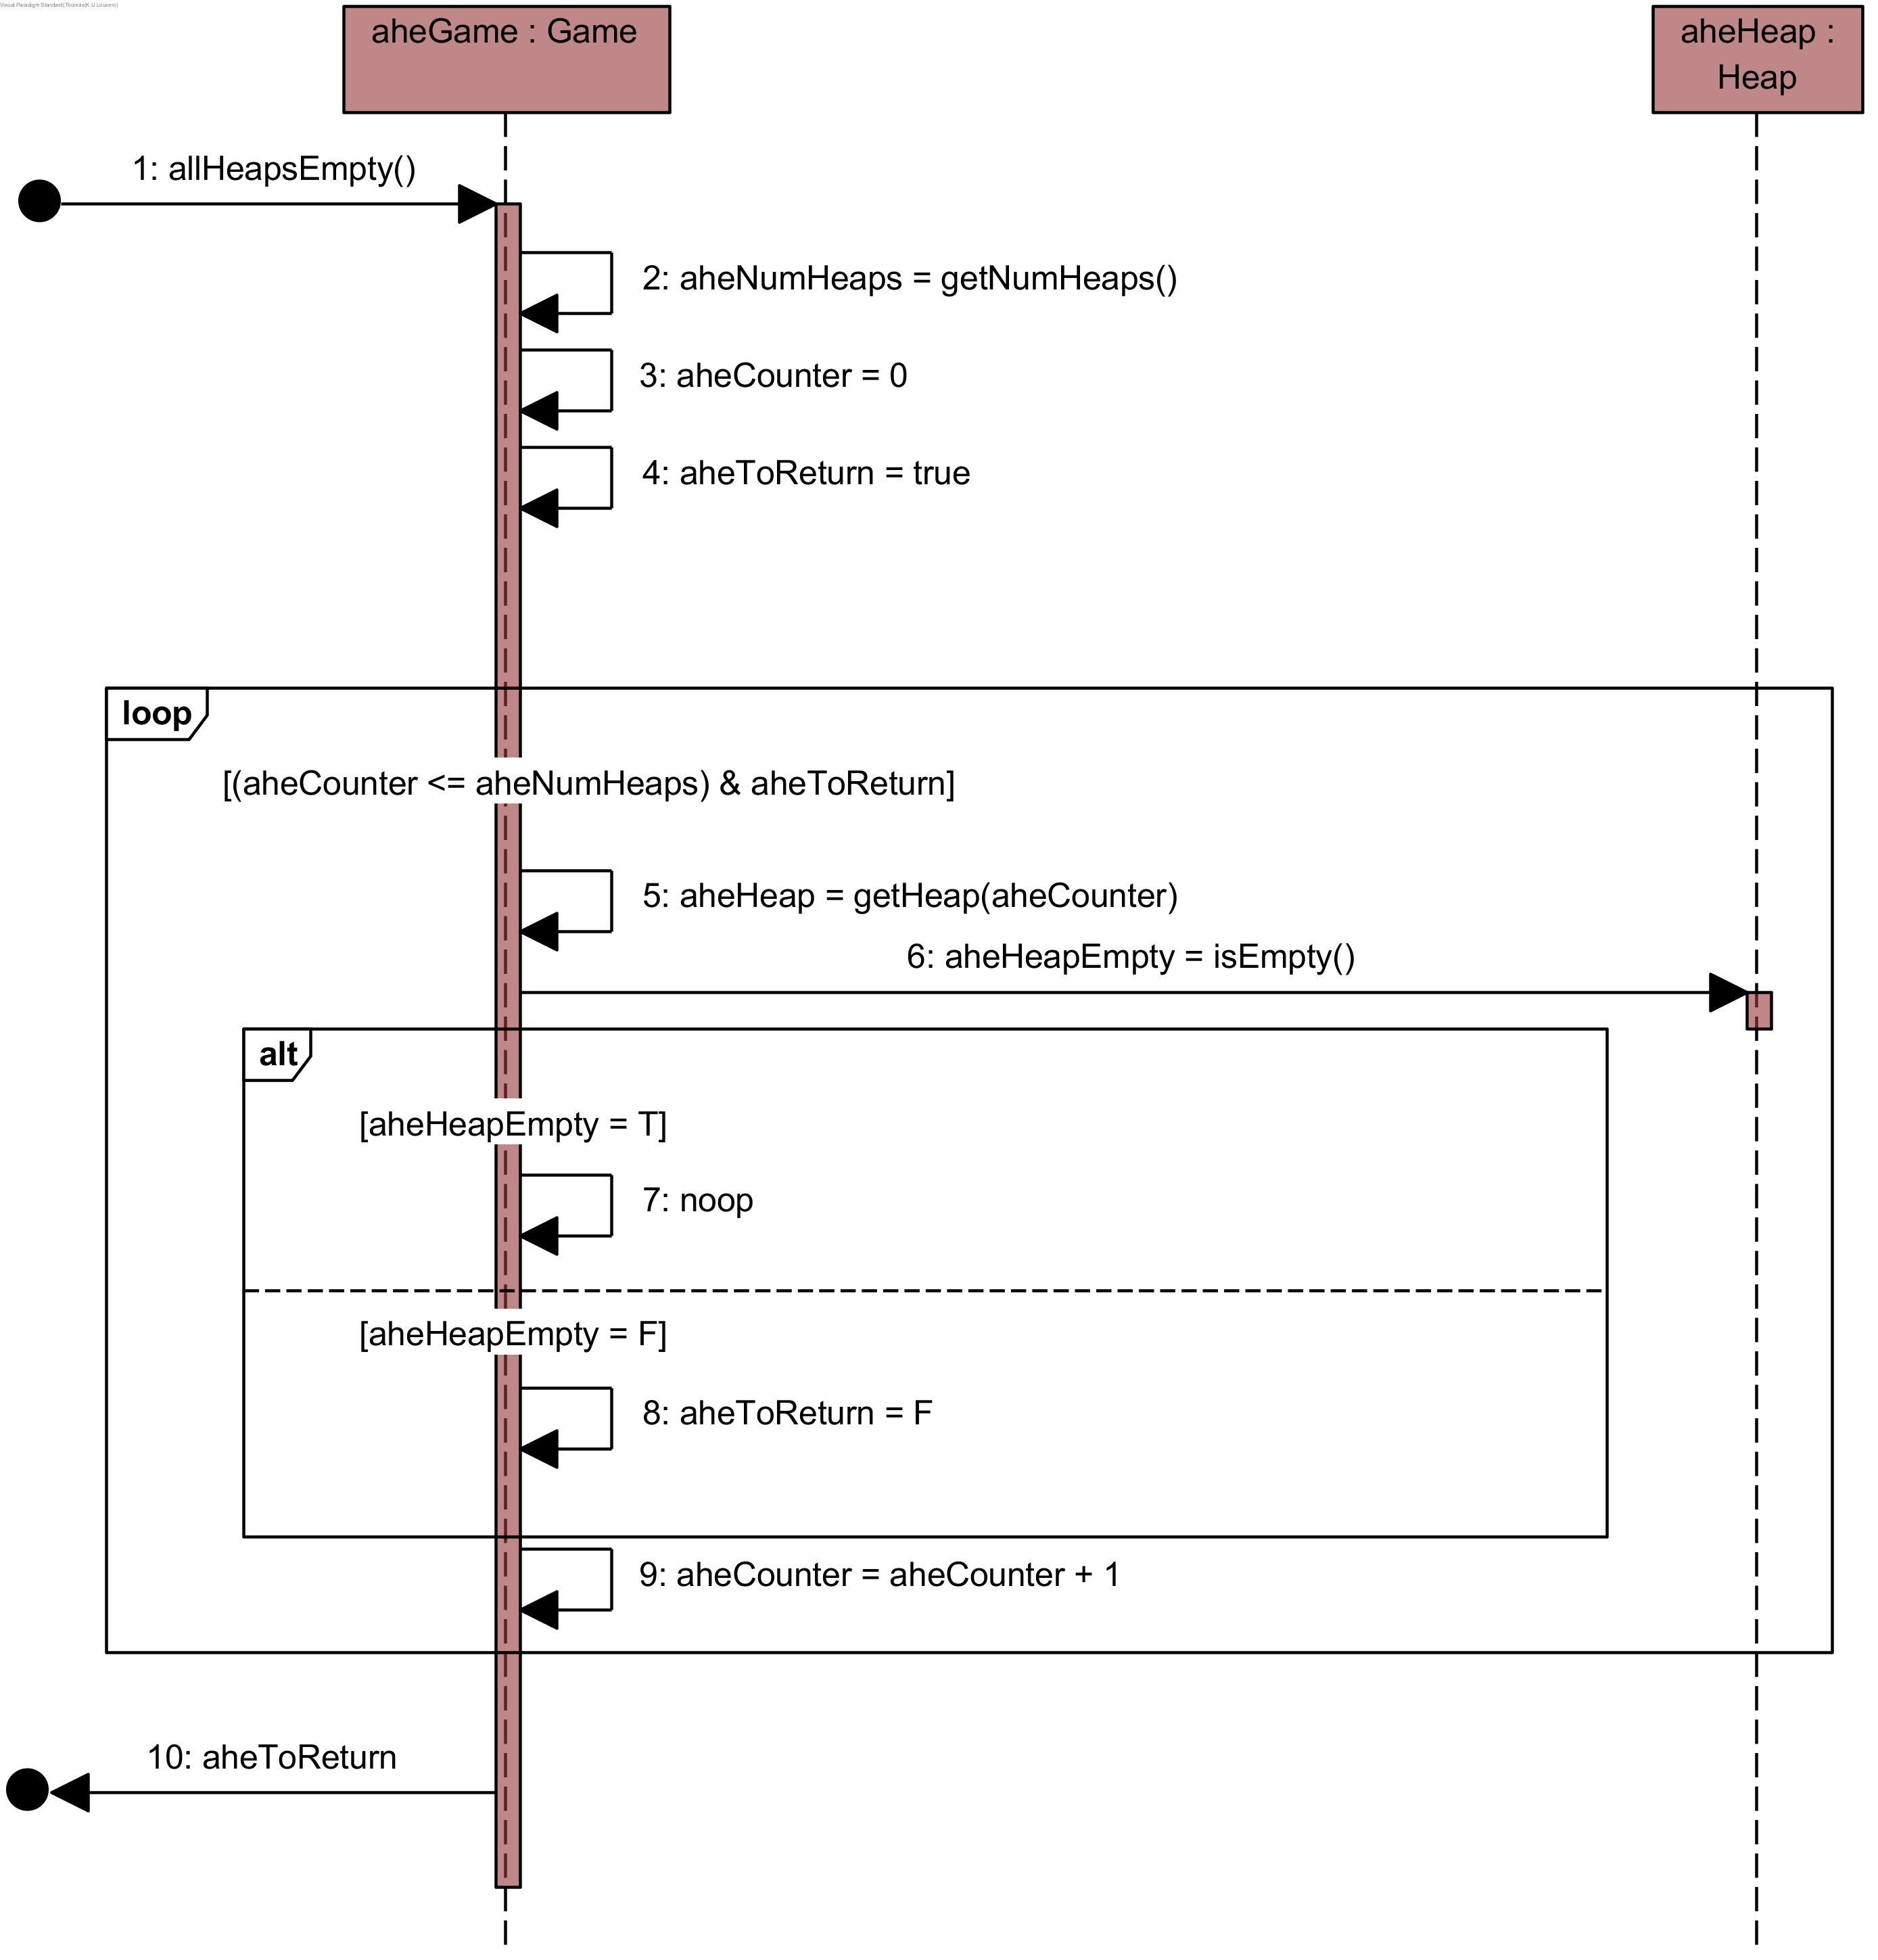
\includegraphics[width=0.6\textwidth]{allHeapsEmpty}%
		\label{fig:ahe}}
	\hfil
	\subfloat[Sequence diagram for \textit{isEmpty()}]{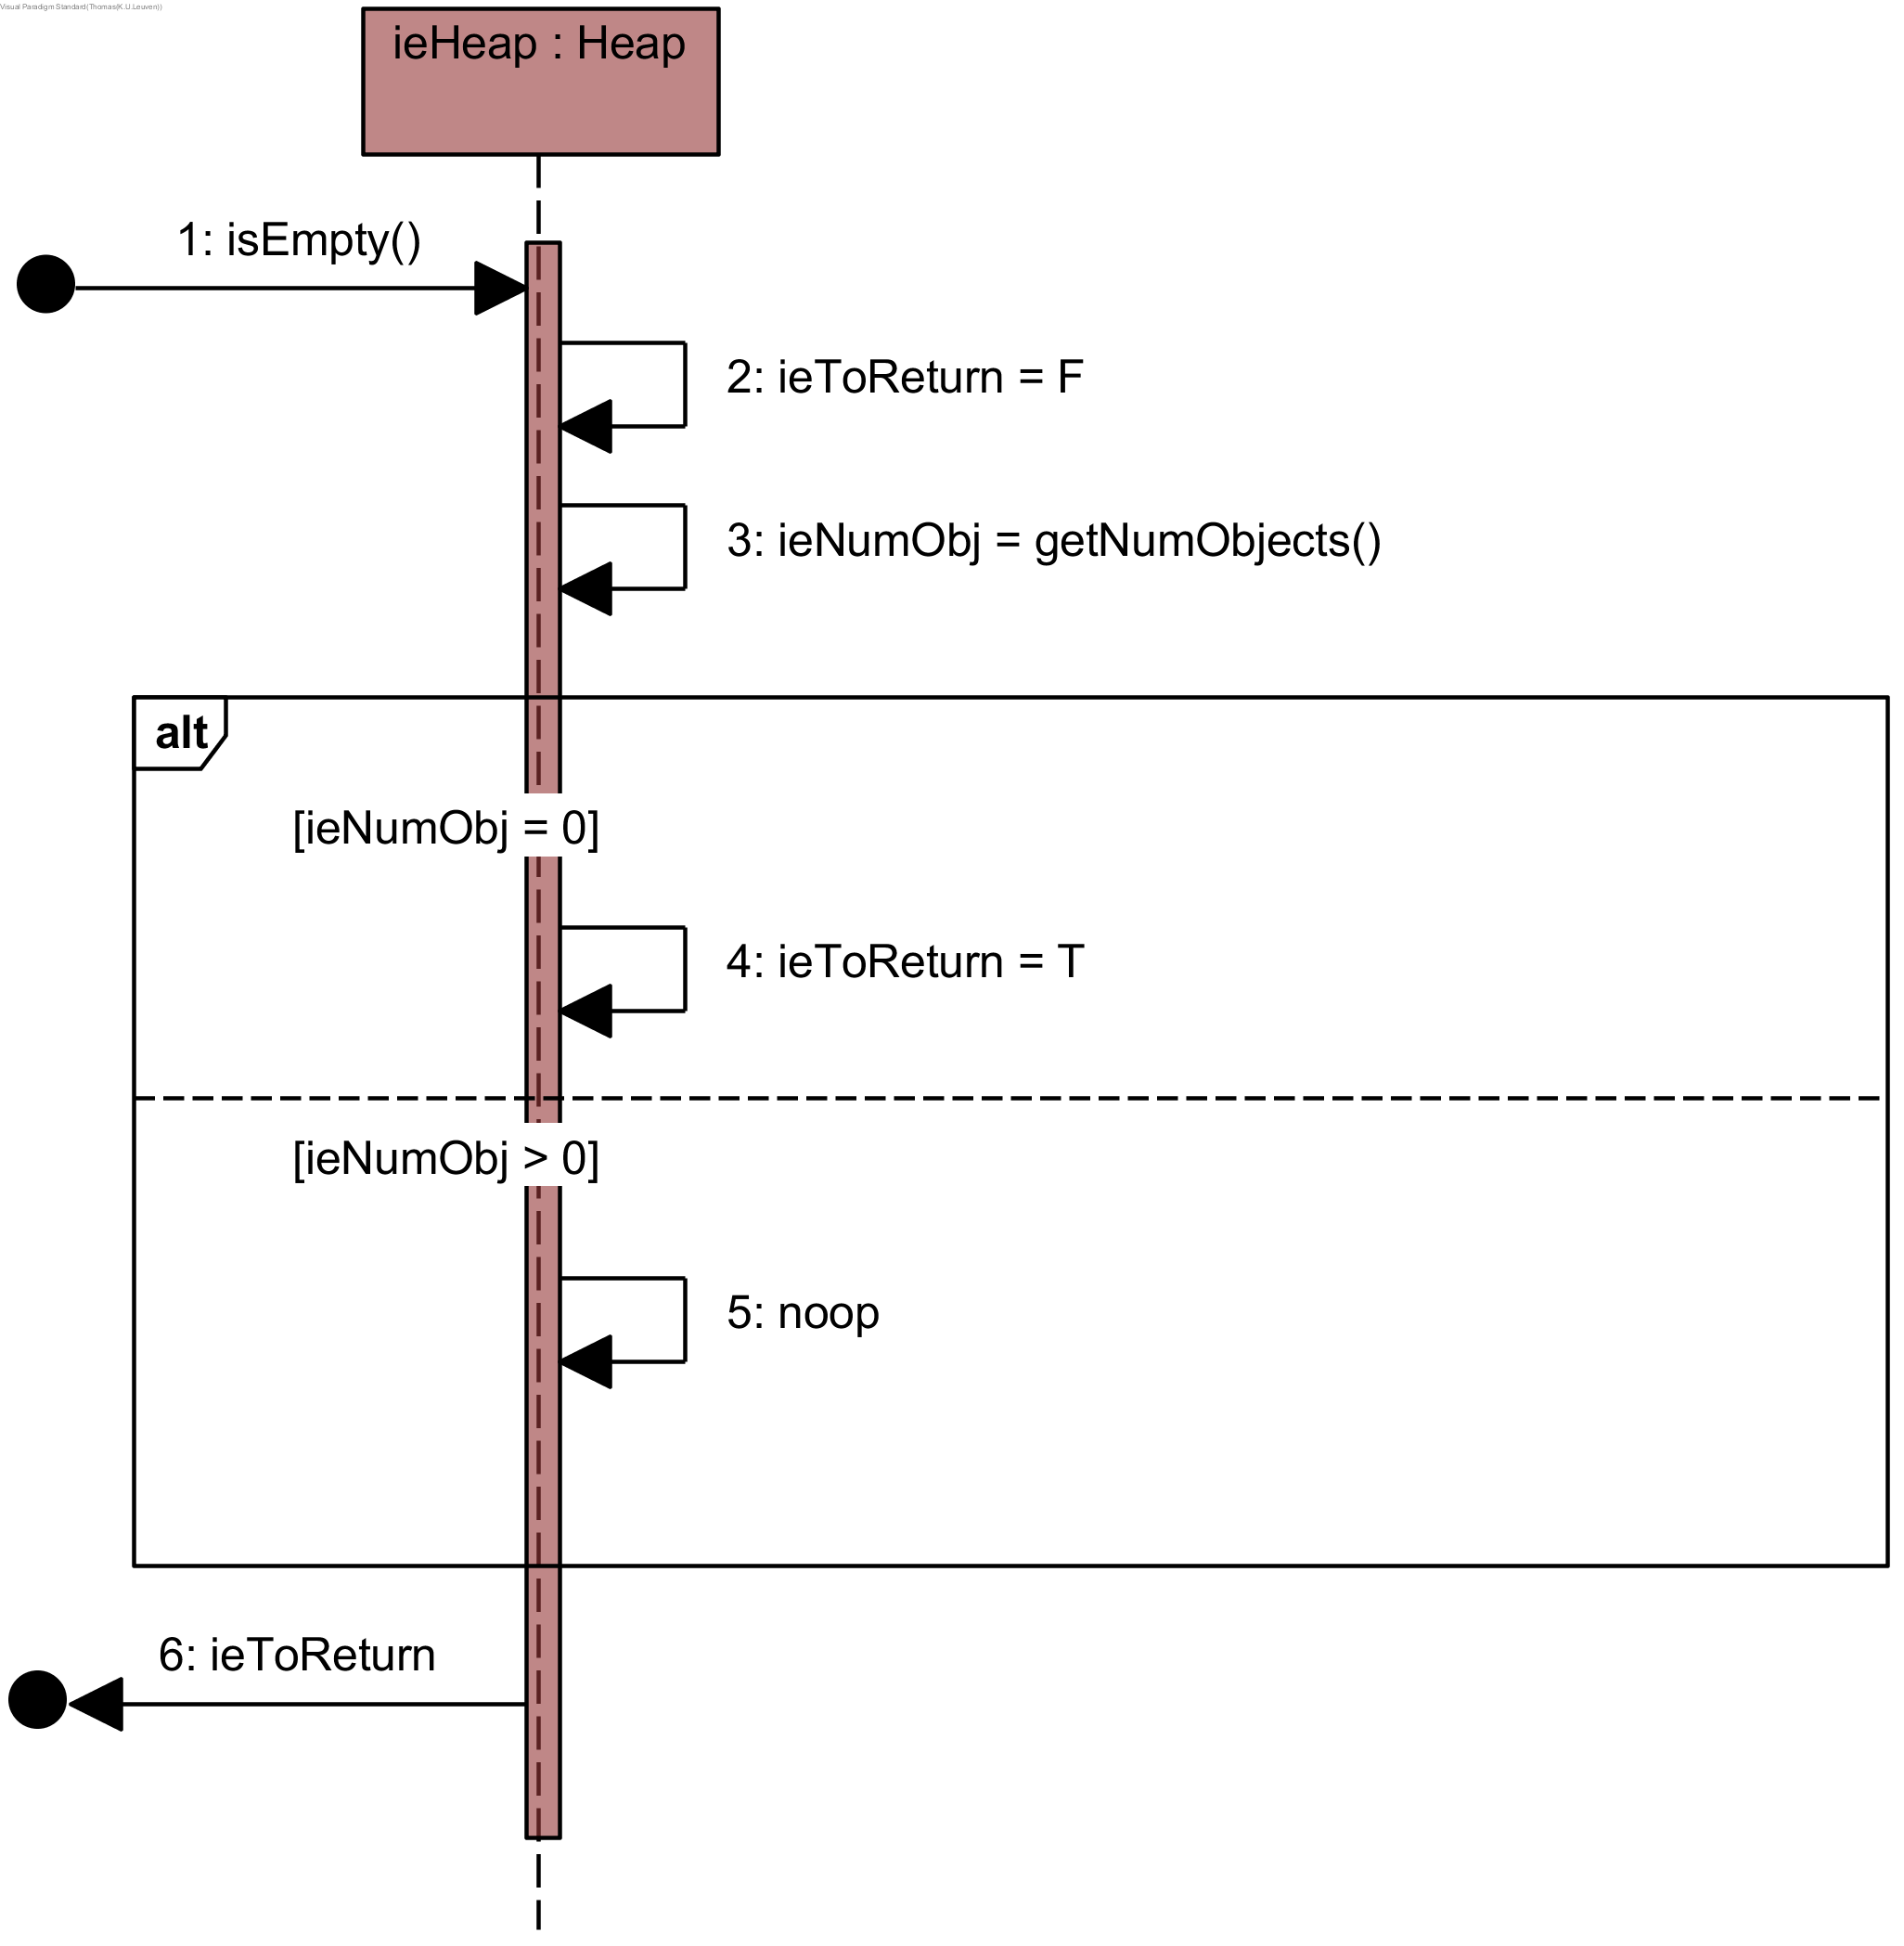
\includegraphics[width=0.4\textwidth]{isEmpty}}%
	\label{fig:isEmpty}
	\caption{Sequence diagrams for \textit{allHeapsEmpty()} and \textit{isEmpty()}}
	\label{fig:ahe-ie}
\end{figure*}

\begin{figure*}[!t]
	\centering
	\subfloat[Sequence diagram from \textit{takeTurn()}]{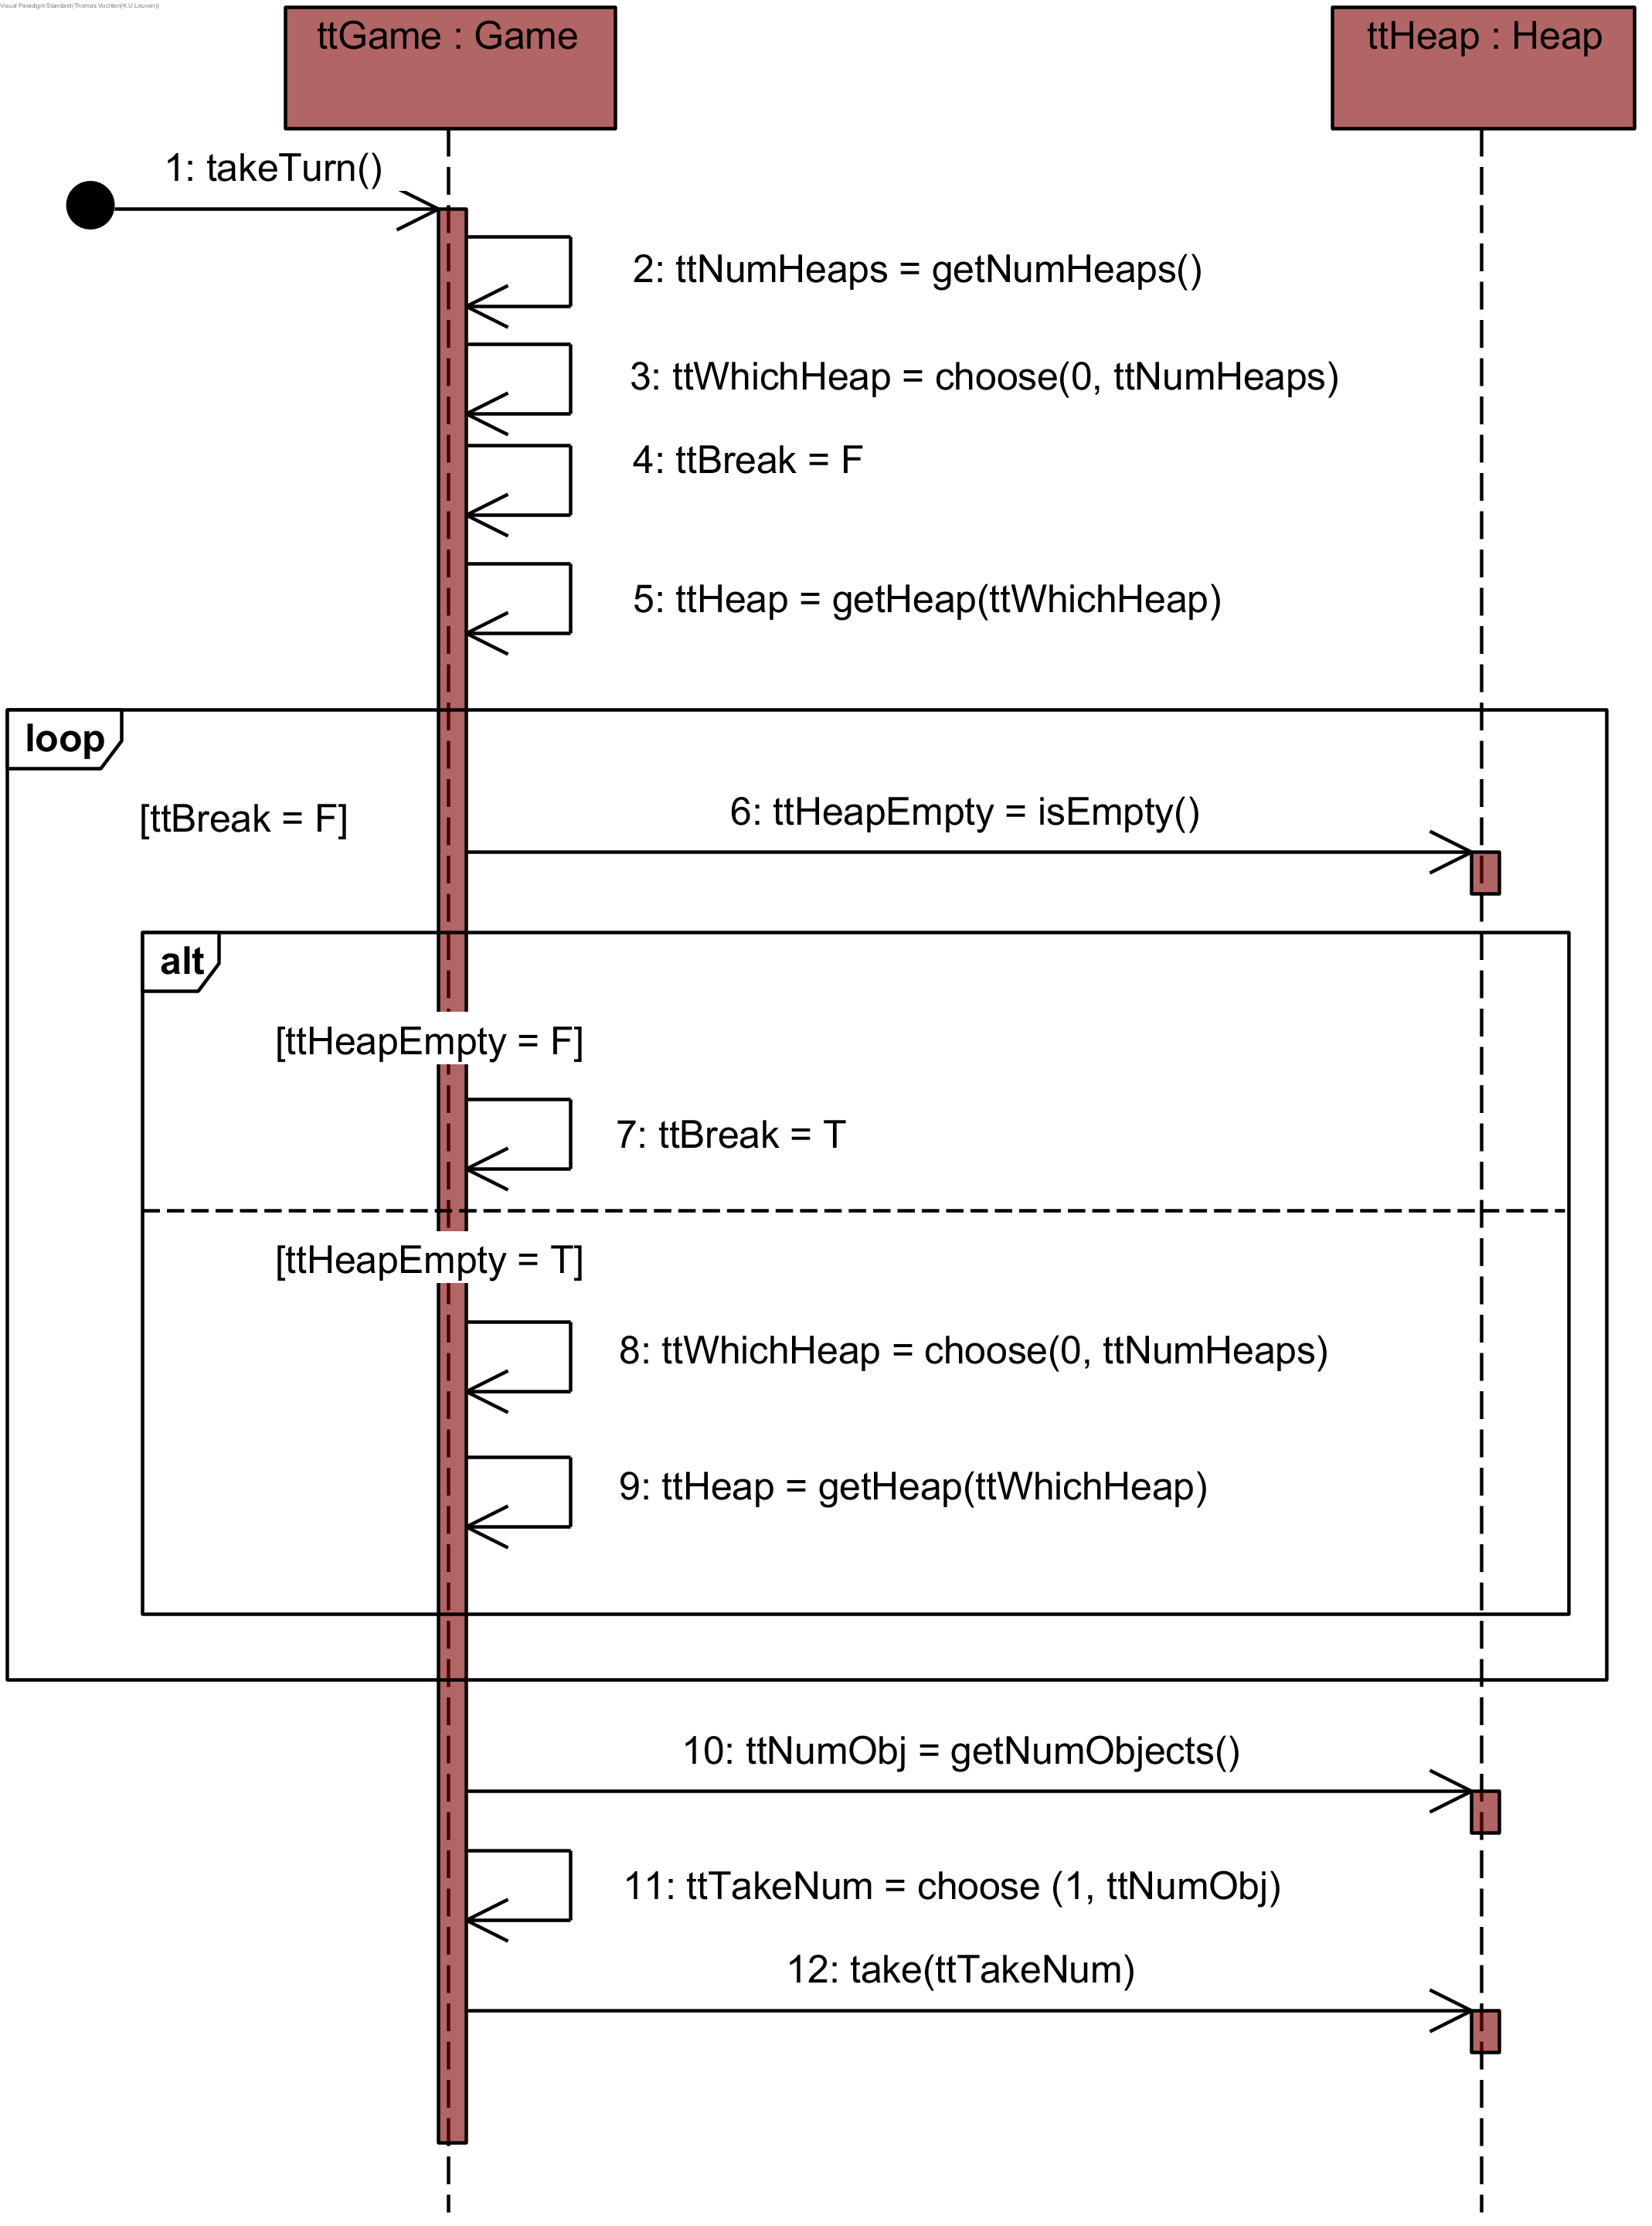
\includegraphics[width=0.5\textwidth]{takeTurn}%
		\label{fig:takeTurn}}
	\hfil
	\subfloat[Sequence diagram for \textit{take(int)}]{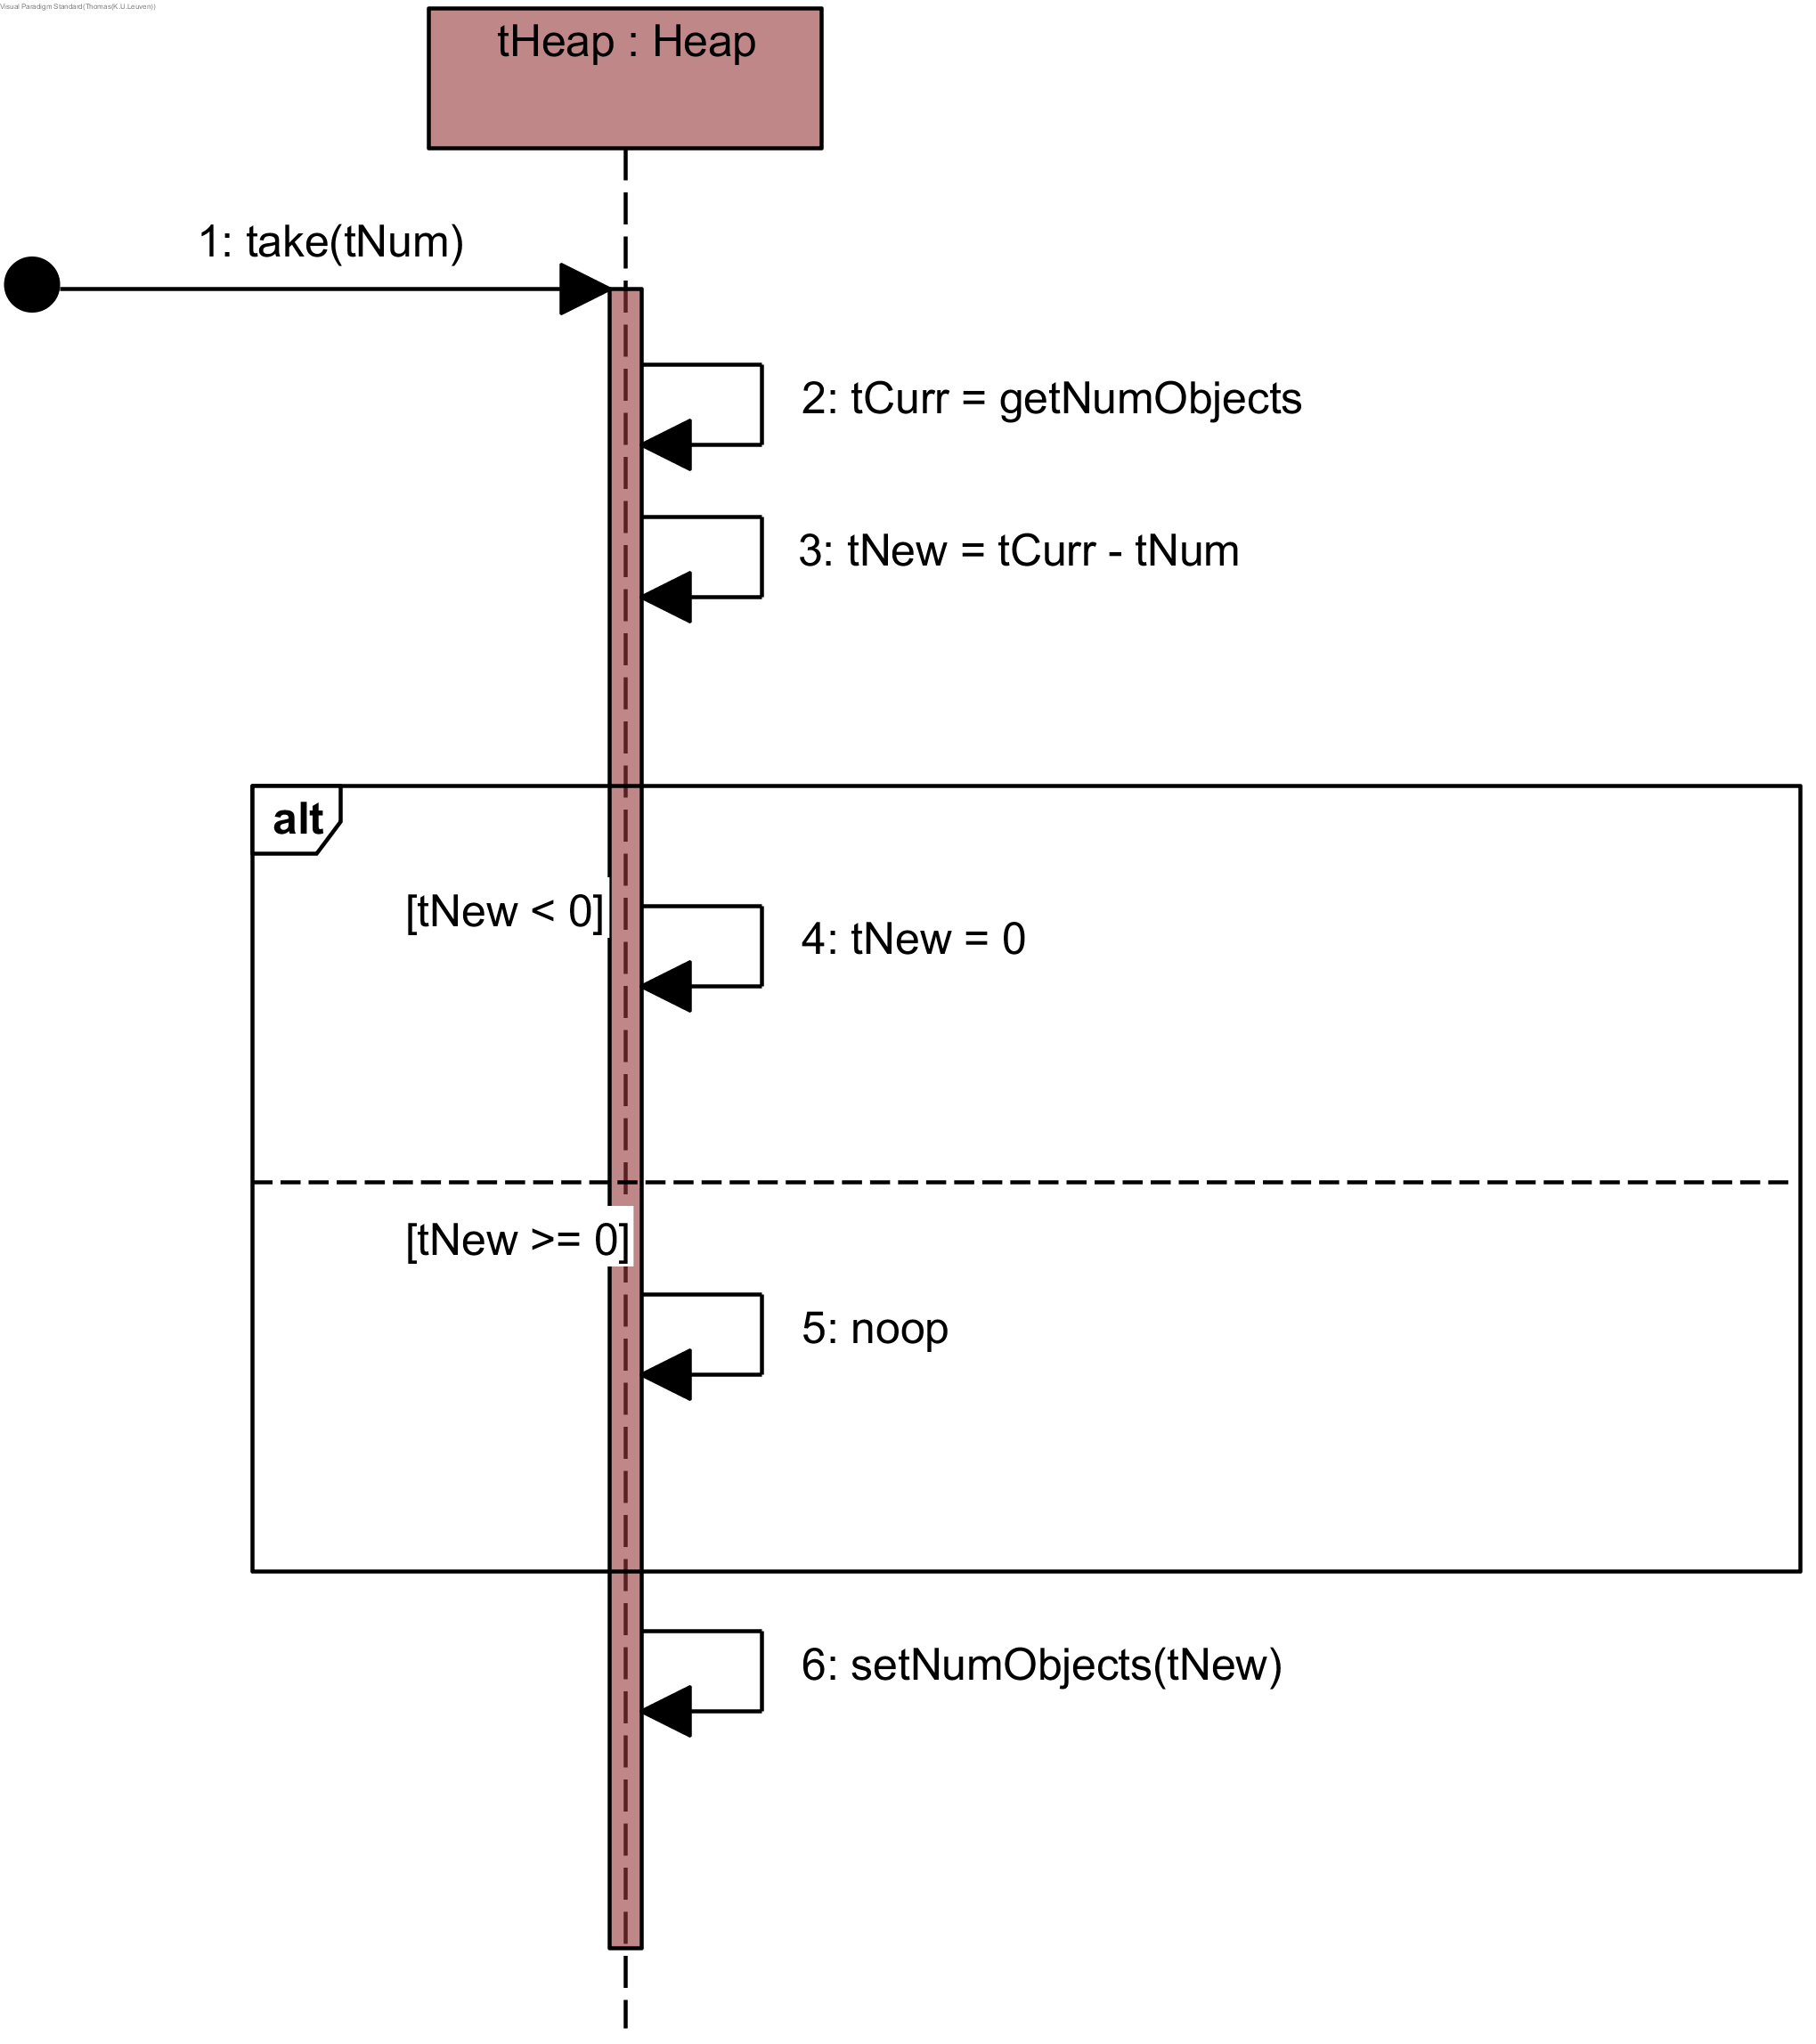
\includegraphics[width=0.5\textwidth]{take}}%
	\label{fig:take}
	\caption{Sequence diagrams for \textit{takeTurn()} and \textit{take(int)}}
	\label{fig:tt-take}
\end{figure*}

\begin{table}[]
	\centering
	\begin{tabular}{|l|l|l|l|l|}
		\hline
		Turn 1 & 0,91 GB  \\ \hline
		Turn 2 & 2,09 GB  \\ \hline
		Turn 3 & 3,34 GB  \\ \hline
		End   & 4,84 GB  \\ \hline
	\end{tabular}
	\caption{Virtual memory usage during the simulation at the start of each turn}
	\label{tab:sim-mem}
\end{table}

\begin{figure*}[!t]
	\centering
	\subfloat[Boxplot of the execution time per simulation step]{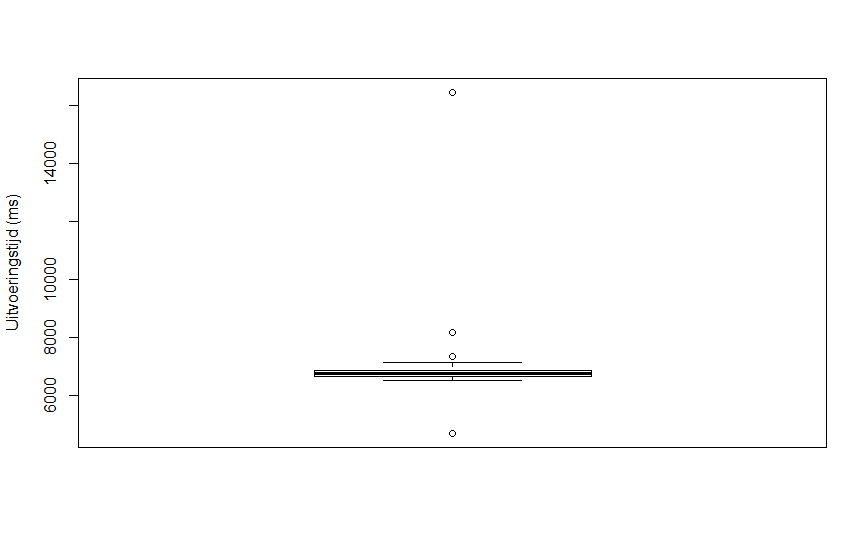
\includegraphics[width=0.5\textwidth]{boxplot}%
		\label{fig:boxplot}}
	\hfil
	\subfloat[Boxplot of the execution time per simulation step with the outliers removed]{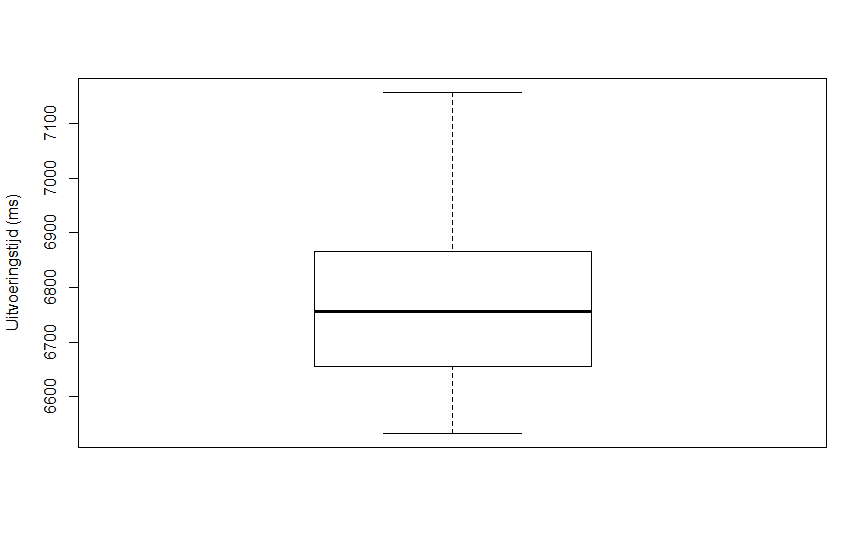
\includegraphics[width=0.5\textwidth]{boxplotnooutliers}}%
		\label{fig:boxplot-nooutliers}
	\caption{Boxplots for the execution time per simulation step}
	\label{fig:boxplots}
\end{figure*}

% An example of a floating figure using the graphicx package.
% Note that \label must occur AFTER (or within) \caption.
% For figures, \caption should occur after the \includegraphics.
% Note that IEEEtran v1.7 and later has special internal code that
% is designed to preserve the operation of \label within \caption
% even when the captionsoff option is in effect. However, because
% of issues like this, it may be the safest practice to put all your
% \label just after \caption rather than within \caption{}.
%
% Reminder: the "draftcls" or "draftclsnofoot", not "draft", class
% option should be used if it is desired that the figures are to be
% displayed while in draft mode.
%
%\begin{figure}[!t]
%\centering
%\includegraphics[width=2.5in]{myfigure}
% where an .eps filename suffix will be assumed under latex, 
% and a .pdf suffix will be assumed for pdflatex; or what has been declared
% via \DeclareGraphicsExtensions.
%\caption{Simulation results for the network.}
%\label{fig_sim}
%\end{figure}

% Note that the IEEE typically puts floats only at the top, even when this
% results in a large percentage of a column being occupied by floats.


% An example of a double column floating figure using two subfigures.
% (The subfig.sty package must be loaded for this to work.)
% The subfigure \label commands are set within each subfloat command,
% and the \label for the overall figure must come after \caption.
% \hfil is used as a separator to get equal spacing.
% Watch out that the combined width of all the subfigures on a 
% line do not exceed the text width or a line break will occur.
%
%\begin{figure*}[!t]
%\centering
%\subfloat[Case I]{\includegraphics[width=2.5in]{box}%
%\label{fig_first_case}}
%\hfil
%\subfloat[Case II]{\includegraphics[width=2.5in]{box}%
%\label{fig_second_case}}
%\caption{Simulation results for the network.}
%\label{fig_sim}
%\end{figure*}
%
% Note that often IEEE papers with subfigures do not employ subfigure
% captions (using the optional argument to \subfloat[]), but instead will
% reference/describe all of them (a), (b), etc., within the main caption.
% Be aware that for subfig.sty to generate the (a), (b), etc., subfigure
% labels, the optional argument to \subfloat must be present. If a
% subcaption is not desired, just leave its contents blank,
% e.g., \subfloat[].


% An example of a floating table. Note that, for IEEE style tables, the
% \caption command should come BEFORE the table and, given that table
% captions serve much like titles, are usually capitalized except for words
% such as a, an, and, as, at, but, by, for, in, nor, of, on, or, the, to
% and up, which are usually not capitalized unless they are the first or
% last word of the caption. Table text will default to \footnotesize as
% the IEEE normally uses this smaller font for tables.
% The \label must come after \caption as always.
%
%\begin{table}[!t]
%% increase table row spacing, adjust to taste
%\renewcommand{\arraystretch}{1.3}
% if using array.sty, it might be a good idea to tweak the value of
% \extrarowheight as needed to properly center the text within the cells
%\caption{An Example of a Table}
%\label{table_example}
%\centering
%% Some packages, such as MDW tools, offer better commands for making tables
%% than the plain LaTeX2e tabular which is used here.
%\begin{tabular}{|c||c|}
%\hline
%One & Two\\
%\hline
%Three & Four\\
%\hline
%\end{tabular}
%\end{table}


% Note that the IEEE does not put floats in the very first column
% - or typically anywhere on the first page for that matter. Also,
% in-text middle ("here") positioning is typically not used, but it
% is allowed and encouraged for Computer Society conferences (but
% not Computer Society journals). Most IEEE journals/conferences use
% top floats exclusively. 
% Note that, LaTeX2e, unlike IEEE journals/conferences, places
% footnotes above bottom floats. This can be corrected via the
% \fnbelowfloat command of the stfloats package.




\section{Conclusion}\label{sec:conclusion}
We have shown how to translate a class diagram and an accompanying set of sequence diagrams that model the behavior of the methods defined in the class diagram to an FO($\cdot$) theory. We have also shown how that theory may be used to verify consistency of the class diagram, to simulate the behavior of the system and to verify requirements on individual diagrams. There is also a translation of a class diagram to an FO($\cdot$) theory in an alternate form. This theory may be used to detect the presence of certain design flaws in a class diagram.

The results from section \ref{sec:evaluation} indicate that execution time and memory usage in terms of grounding size are already high even for diagrams that model simple games such as Nim. The way forward would be to find ways to make the output theory as small as possible. The most promising avenue would likely be to introduce declarative elements to the modelling language of sequence diagrams. Examples would be an instruction that extracts all elements that satisfy a query from a variable representing a collection and an instruction that allows the user to choose one or more elements that satisfy a query from a collection during simulation.


% conference papers do not normally have an appendix


% use section* for acknowledgment
%\section*{Acknowledgment}
%
%
%The authors would like to thank...





% trigger a \newpage just before the given reference
% number - used to balance the columns on the last page
% adjust value as needed - may need to be readjusted if
% the document is modified later
%\IEEEtriggeratref{8}
% The "triggered" command can be changed if desired:
%\IEEEtriggercmd{\enlargethispage{-5in}}

% references section

% can use a bibliography generated by BibTeX as a .bbl file
% BibTeX documentation can be easily obtained at:
% http://mirror.ctan.org/biblio/bibtex/contrib/doc/
% The IEEEtran BibTeX style support page is at:
% http://www.michaelshell.org/tex/ieeetran/bibtex/
\bibliographystyle{IEEEtran}
% argument is your BibTeX string definitions and bibliography database(s)
\bibliography{citations}{}
%
% <OR> manually copy in the resultant .bbl file
% set second argument of \begin to the number of references
% (used to reserve space for the reference number labels box)
%\begin{thebibliography}{1}
%
%\bibitem{IEEEhowto:kopka}
%H.~Kopka and P.~W. Daly, \emph{A Guide to \LaTeX}, 3rd~ed.\hskip 1em plus
%  0.5em minus 0.4em\relax Harlow, England: Addison-Wesley, 1999.
%
%\end{thebibliography}

% that's all folks
\end{document}




\chapter{Poster}

\includepdf[pages=1,fitpaper]{postera4.pdf}